%%
%% Copyright 2007-2019 Elsevier Ltd
%%
%% This file is part of the 'Elsarticle Bundle'.
%% ---------------------------------------------
%%
%% It may be distributed under the conditions of the LaTeX Project Public
%% License, either version 1.2 of this license or (at your option) any
%% later version.  The latest version of this license is in
%%    http://www.latex-project.org/lppl.txt
%% and version 1.2 or later is part of all distributions of LaTeX
%% version 1999/12/01 or later.
%%
%% The list of all files belonging to the 'Elsarticle Bundle' is
%% given in the file `manifest.txt'.
%%

%% Template article for Elsevier's document class `elsarticle'
%% with numbered style bibliographic references
%% SP 2008/03/01
%%
%%
%%
%% $Id: elsarticle-template-num.tex 164 2019-01-14 09:57:55Z rishi $
%%
%%
%%\documentclass[preprint,12pt]{elsarticle}

%% Use the option review to obtain double line spacing
%% \documentclass[authoryear,preprint,review,12pt]{elsarticle}

%% Use the options 1p,twocolumn; 3p; 3p,twocolumn; 5p; or 5p,twocolumn
%% for a journal layout:
%% \documentclass[final,1p,times]{elsarticle}
%% \documentclass[final,1p,times,twocolumn]{elsarticle}
%% \documentclass[final,3p,times]{elsarticle}
\documentclass[final,3p,times,twocolumn]{elsarticle}
%% \documentclass[final,5p,times]{elsarticle}
%%%\documentclass[final,5p,times,twocolumn]{elsarticle}

%% For including figures, graphicx.sty has been loaded in
%% elsarticle.cls. If you prefer to use the old commands
%% please give \usepackage{epsfig}

%% The amssymb package provides various useful mathematical symbols
\usepackage{amssymb}
%% The amsthm package provides extended theorem environments
%% \usepackage{amsthm}
\usepackage{amsmath}
\usepackage{indentfirst}
\usepackage{epsfig}
\usepackage{ulem}
% \usepackage{epstopdf}
\usepackage{listings}
\usepackage{subfig}
\usepackage{lipsum}
\usepackage{color}
\usepackage{soul}
%\usepackage[lined,algonl,ruled]{algorithm2e}
% \usepackage{subfigure}
\usepackage{graphicx}
\usepackage[T1]{fontenc}
\newcommand{\secref}[1]{Section \ref{#1}}
\newcommand{\figref}[1]{Figure \ref{#1}}
\newcommand{\tabref}[1]{Table \ref{#1}}
\newcommand{\equref}[1]{Equation (\ref{#1})}
% \renewcommand{\algorithmicrequire}{\textbf{Input:}}
% \renewcommand{\algorithmicensure}{\textbf{Output:}}
\newcommand{\KZ}[1]{\textcolor{red}{[Kenny: #1]}}
%\newcommand{\JY}[1]{\textcolor{blue}{[Jinyi: #1]}}
\newcommand{\KQ}[1]{\textcolor{red}{#1}}
\lstset{
  captionpos=b,
  tabsize=2,
  % numbers=left,
  % numberstyle=\tiny,
  % numbersep=5pt,
  breaklines=true,
  showstringspaces=true,
  basicstyle=\small,
  frame=none,
  emph={label},
  escapechar=* % Escape to LaTeX between |...|
}
%% The lineno packages adds line numbers. Start line numbering with
%% \begin{linenumbers}, end it with \end{linenumbers}. Or switch it on
%% for the whole article with \linenumbers.
%% \usepackage{lineno}

\journal{Computers in Biology and Medicine}

\begin{document}

\begin{frontmatter}

%% Title, authors and addresses

%% use the tnoteref command within \title for footnotes;
%% use the tnotetext command for theassociated footnote;
%% use the fnref command within \author or \address for footnotes;
%% use the fntext command for theassociated footnote;
%% use the corref command within \author for corresponding author footnotes;
%% use the cortext command for theassociated footnote;
%% use the ead command for the email address,
%% and the form \ead[url] for the home page:
%% \title{Title\tnoteref{label1}}
%% \tnotetext[label1]{}
%% \author{Name\corref{cor1}\fnref{label2}}
%% \ead{email address}
%% \ead[url]{home page}
%% \fntext[label2]{}
%% \cortext[cor1]{}
%% \address{Address\fnref{label3}}
%% \fntext[label3]{}

\title{Layout-aware Information Extraction from Semi-structured Medical Images}

%% use optional labels to link authors explicitly to addresses:
%% \author[label1,label2]{}
%% \address[label1]{}
%% \address[label2]{}

\author[sjtu]{Kangqi Luo}
\author[sjtu]{Jinyi Lu}
\author[sjtu]{Kenny Q. Zhu\corref{cor1}}
\ead{kzhu@cs.sjtu.edu.cn}

\author[az]{Weiguo Gao}
\author[az]{Jia Wei\corref{cor1}}
\ead{jenny.wei@astrazeneca.com}
\author[az]{Meizhuo Zhang}

\address[sjtu]{Shanghai Jiao Tong University, 800 Dongchuan Road, Shanghai 200240, P.R. China}
\address[az]{AstraZeneca China, 199 Liangjing Road, Shanghai 201203, P.R. China}

\cortext[cor1]{Corresponding authors.}

\begin{abstract}
\st{
Digitizing paper documents and extracting structured information is an
important part of information retrieval and knowledge discovery.
Optical character recognition (OCR) has been widely used
in this task, and achieved promising results on textual documents
%and promising results have been achieved in applying OCR to textual documents,
such as books and reports.
For the ultimate goal of building electronic medical records,
the textual information embedded in the medical image
contains rich structured knowledge of the particular patient.
% For %semi-structured
% medical images that combine graphics and words,
However, due to the discontinuity of text flows,
%extraction of useful textual information is difficult
extracting structured textual data from medical images becomes more challenging.
}
\KQ{
Textual information embedded in the medical image
contains rich structured information about the medical condition of a patient.
This paper aims at extracting structured textual information from semi-structured medical images.
Given the recognized text spans of an image preprocessed by
optical character recognition (OCR),
due to the spatial discontinuity of texts spans
as well as potential errors brought by OCR,
the structured information extraction becomes more challenging.
}
In this paper, we propose a
domain-specific language, called ODL, which allows users to describe
the value and layout of text data contained in the images.
Based on the value and spatial constraints described in ODL,
the ODL parser
\st{parses the raw OCR output of the medical image into a parse tree, and}
associates values found in the image with the data structure in the
ODL description, while conforming to the aforementioned constraints.
\st{
Robustness is the major advantage during this parsing process,
as the parser doesn't rely on carefully annotated bounding boxes
of structured data in the medical image,
and is able to tolerate or even automatically correct some of the errors
introduced by OCR.
Compared with baseline methods in the same task,
our ODL parser shows the better tolerance of positional variances between
images, and consistently outperforms existing approaches in terms of
extraction accuracy.
}
\KQ{
We conduct experiments on a dataset consisting of real medical images,
our ODL parser consistently outperforms existing approaches in terms of
extraction accuracy,
which shows the better tolerance of incorrectly recognized texts,
and positional variances between images.}
This accuracy can be further improved by learning from a few manual corrections.

\end{abstract}

\begin{keyword}
%% keywords here, in the form: keyword \sep keyword
information extraction \sep
medical images \sep
electronic medical records \sep
domain-specific language \sep
spatial layout \sep
optical character recognition

%% PACS codes here, in the form: \PACS code \sep code

%% MSC codes here, in the form: \MSC code \sep code
%% or \MSC[2008] code \sep code (2000 is the default)

\end{keyword}

\end{frontmatter}

%% \linenumbers
\section{Introduction}
\label{sec:intro}

% Part 1: Text IE, scenarios, OCR
% What is text information extraction?
Information extraction is the task of automatically extracting information
or knowledge from unstructured or semi-structured documents.
In the domain of image processing,
the task of textual information extraction (TIE)
is automatically detecting and recognizing texts from given images.
% where is it used?
TIE is applied in a large variety of image categories,
such as printed books, newspapers, digital drawings,
or even more general images~\cite{jung2004text}.
% What's the kernel technique?
Optical character recognition (OCR) is the popular approach to solve TIE,
turning images of printed text into machine encoded texts.
OCR is a hot research topic in recent years, and the performance is promising
on \st{plain-text-based images} \KQ{images containing largely text},
such as novels and reports.
For example, Tesseract~\cite{smith2007overview},
one of the most popular open source multilingual recognizers,
achieved an error rate of 3.72\% for recognizing English words
and 3.77\% for simplified Chinese characters\cite{smith2009adapting}.
Based on the exclusive use and high accuracy of OCR,
the Google Books~\cite{vincent2007google} and Gutenberg Project~\cite{lebert2008project}
have scanned a large number of printed books
and converted into text for free and open access.

\begin{figure*}[!htb]
\centering
\subfloat[ECG]{
\label{fig:medicalimage:ecg}
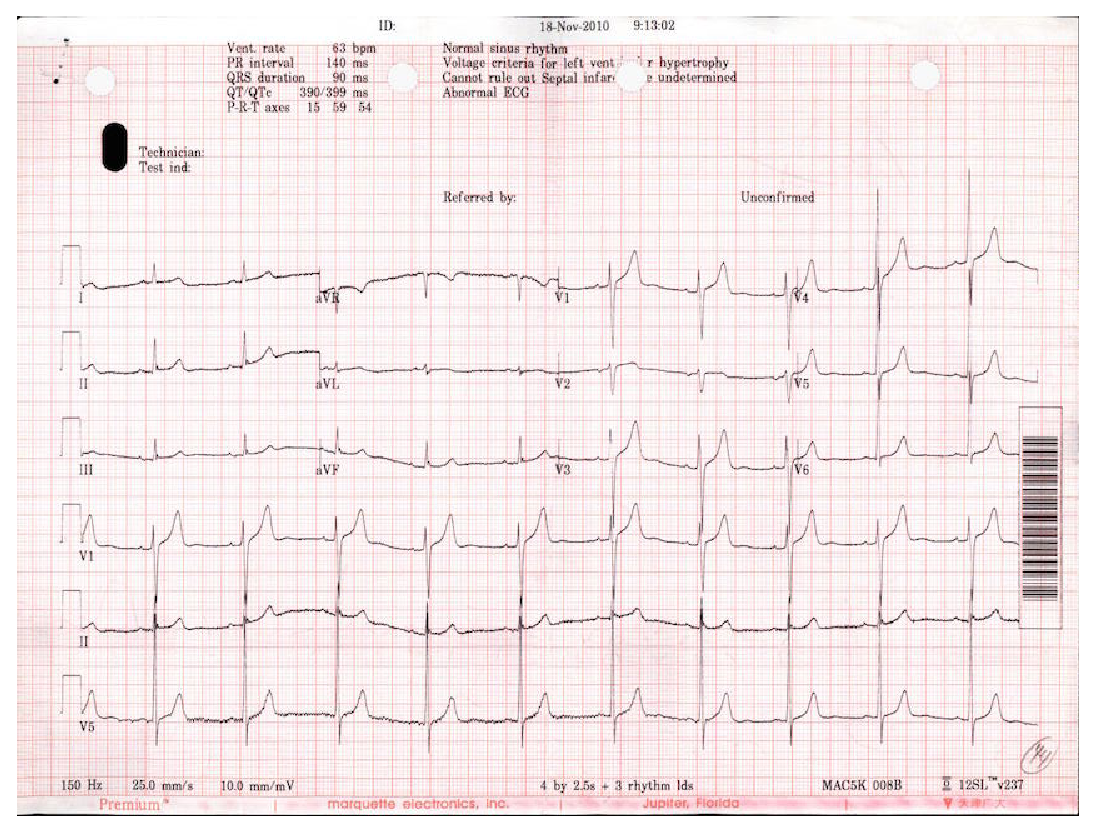
\epsfig{file=figure/ECG.eps, width=1.10\columnwidth}
}
% % \hfill
% \subfloat[X-RAY]{
% \label{fig:medicalimage:xray}
% \epsfig{file=figure/X-RAY.eps, width=0.4\columnwidth}
% }
% \hfill
\subfloat[MRI]{
\label{fig:medicalimage:mrt}
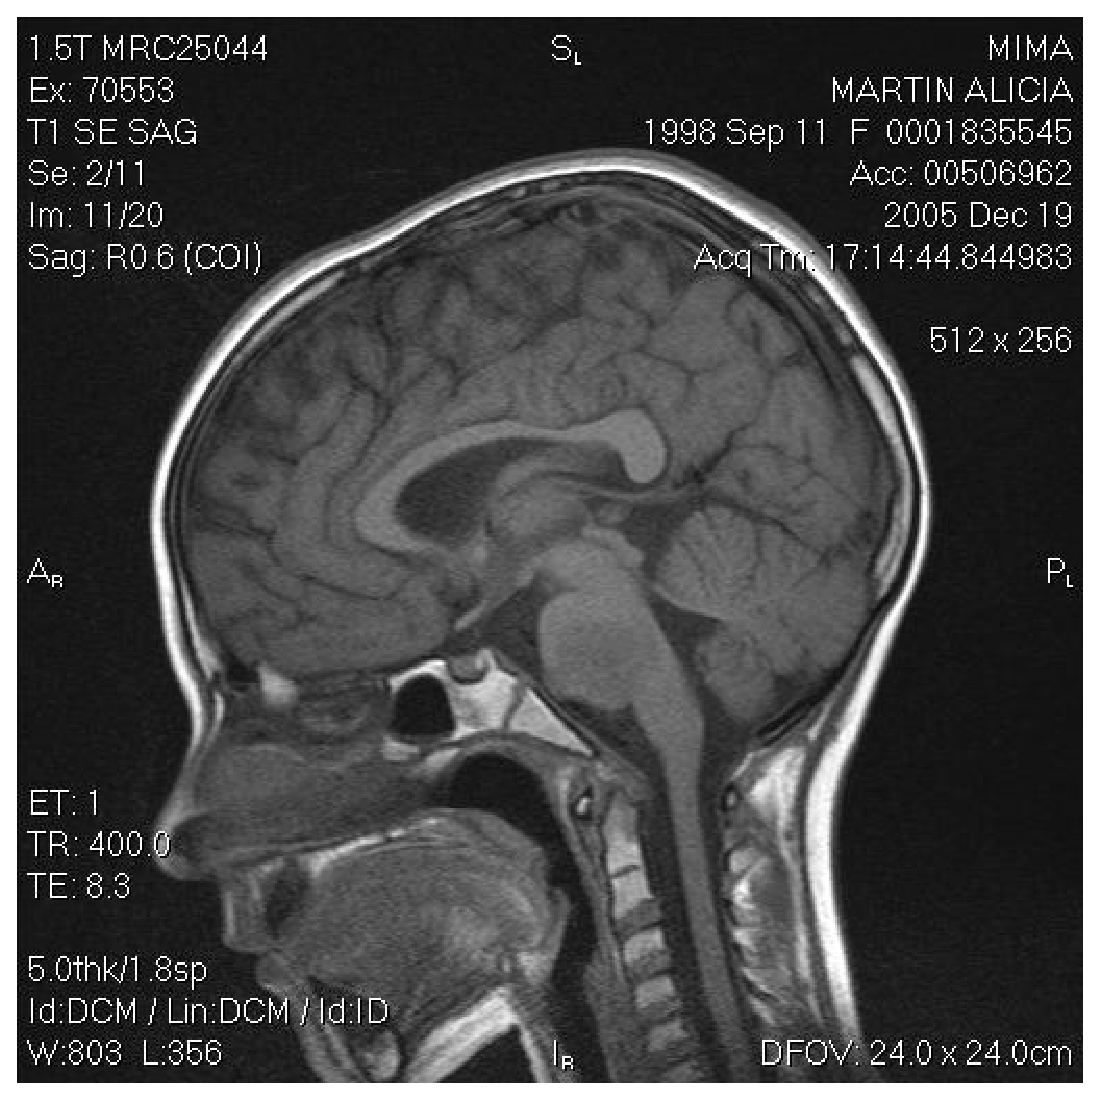
\epsfig{file=figure/MRI.eps, width=0.88\columnwidth}
}
% \subfloat[EEG]{
% \label{fig:medicalimage:eeg}
% 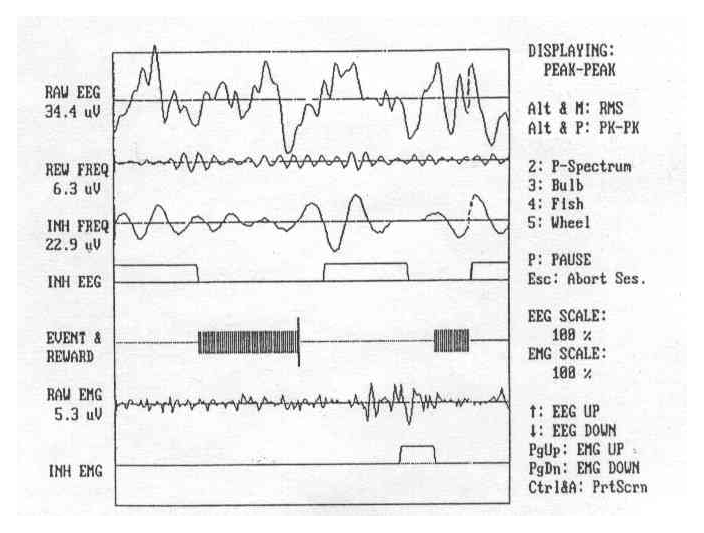
\epsfig{file=figure/EEG.eps, width=0.4\columnwidth}
% }
\caption{Examples of medical images with textual information.}
\label{fig:med-image-example}
\end{figure*}


% Part 2: Medical imaging, example image, raw OCR result (text + layout information)
% What's medical image, why important?
Due to ever evolving hardware and software, many medical images
such as electro-cardio graphs (ECGs), magnetic resonance imaging (MRI),
X-ray or ultrasound images are directly printed and stored
\st{in hard copy formats} \KQ{on paper}.
Medical images shown in \figref{fig:med-image-example}
contain a mix of graphics and text,
which include technical settings of the hardware used,
test measurements and simple diagnoses.
% TODO: why growing demand?
In order to build the manageable electronic medical records for patients,
there has been a growing demand for extracting such text-based
medical information from these medical images.
% What's the exmaple, and what's in the OCR output?
Given the ECG image in \figref{fig:running-ecg} as the running example,
existing OCR softwares are able to produce texts with spatial layout information,
indicating the positions of each recognized text in the image.
\figref{fig:running-xml} shows the raw OCR result produced by Tesseract,
where recognized texts are organized in the form of XML hierarchy of spans,
and we call them ``text boxes'' throughout this paper.
Texts are stored only in leaf text boxes,
and the layout information of each box is represented by
the coordinates (left, top, right, bottom) of its bounding box.
We use the term ``bounding box'' and ``zone'' interchangeably in this paper.
% TODO: Mention OCR error here??
It's worth mentioning that OCR softwares may generate incorrect texts.
for example, the original text ``Vent. rate'' in the image
is incorrectly recognized as ``Vcnt. rule'',
also ``63 bpm'' is recognized as ``53 bpm''.

\begin{figure*}[ht]
\centering
\epsfig{file=figure/running_ECG.eps, width=1.9\columnwidth}
\caption{An ECG with interesting text areas marked by red ovals.}
\label{fig:running-ecg}
\end{figure*}

% \begin{figure}[ht]
% \centering
% \subfigure[]{
% \label{fig:subfig:a}
% \begin{minipage}[b]{0.2\textwidth}
%\newsavebox{\firstlisting}
%\begin{lrbox}{\firstlisting}% Store first listing
%\begin{lstlisting}
%<p class='ocr_par' dir='ltr'>
%   <span class='ocr_line' id='line_2'>
%       <span class='ocrx_word' id='word_6'>Vent.</span> 
%       <span class='ocrx_word' id='word_7'>rate</span> 
%       <span class='ocrx_word' id='word_8'>65</span> 
%       <span class='ocrx_word' id='word_9'>bpm</span> 
%   </span>
%   <span class='ocr_line' id='line_3'>
%       <span class='ocrx_word' id='word_14'>PR</span> 
%       <span class='ocrx_word' id='word_15'>interval</span> 
%       <span class='ocrx_word' id='word_16'>162</span> 
%       <span class='ocrx_word' id='word_17'>ms</span> 
%   </span>
%    ...
%</p> 
%\end{lstlisting}
%\end{lrbox}
% \end{minipage}
% }
% \hspace[1in]
% \subfigure[]{
% % \label{fig:subfig:b}
% % \begin{minipage}[b]{0.2\textwidth}
\newsavebox{\secondlisting}
\begin{lrbox}{\secondlisting}
% \tiny
\begin{lstlisting}[basicstyle=\tiny,]
<p class="ocr_par" title="box 263 33 444 119">
   <span class="ocr_l" title="box 264 33 336 45">
       <span class="ocrx_w" title="box 264 33 299 45">Vcnt.</span> 
       <span class="ocrx_w" title="box 308 34 336 45">rule</span> 
   </span>
   <span class='ocr_l'>
       <span class="ocrx_w" title="box 264 51 283 64">PR</span> 
       <span class="ocrx_w" title="box 291 51 346 64">Interval</span> 
       <span class="ocrx_w" title="box 389 52 411 64">140</span> 
       <span class="ocrx_w" title="box 420 55 439 64">ms</span> 
   </span>
   ...
   </span>
</p>
<p class="ocr_p" dir="ltr">
   <span class="ocr_l">
       <span class="ocrx_w" title="box 396 33 411 45">53</span> 
       <span class="ocrx_w" title="box 420 33 449 48">bpm</span> 
   </span>
</p>
\end{lstlisting}
\end{lrbox}
% % \end{minipage}
% }

% \KZ{\figref{fig:ocrre} is output from what software? Tesseract?}
\begin{figure}[th]
%\subfloat[Image From Printer1]{
%\label{fig:ocrresub:a}
%\scalebox{0.8}{\usebox{\firstlisting}}} 
%\hfill
%\subfloat[Image From Printer2]{
\scalebox{0.6}{\usebox{\secondlisting}}
% \label{fig:ocrre}
\caption{Simplified OCR Results in XML for an ECG with Layout Information}
%\label{fig:ocrresub:b}
\label{fig:ocrre}
\end{figure}

% \lipsum[2]



% Part 3: Goal of this paper: structured information (kv pair) extraction
%         Challenge: hard to write wrapper (professional, not friendly)
%                    noisy information & OCR error
%         direct approach: zonal approaches
%         weakness: error propagation
% kernel: structure --> pure OCR (text, regex based approach) is not reliable: not in a same box
% ZOI approach: zonal / page layout: inaccurate position (between diff. figures), error propagation

% What's the final goal?
Apart from scanning the images into digital formats,
extracting the structured textual knowledge is more important for
building electronic medical records.
% Using examples to illustrate.
For example in \figref{fig:running-ecg},
we would like to extract the attribute-value pairs
(e.g., \textit{Vent. rate = 63 bpm}) and possibly other values such as
date (e.g., \textit{18-Nov-2010}) and time (e.g., \textit{9:13:02}),
since those values endow us with information of the particular patient.
% Informally define the task
% Obviously, raw OCR results didn't explicitly encode such structured knowledge,
Since discovering structured knowledge is beyond the scope of the OCR techniques,
the goal of this work is to provide a systematic solution,
which enables users to easily specify the data of interest in the images,
and automatically extract the corresponding textual values from raw OCR results.

There are some naive solutions for this information extraction task.
% Naive approach 1: regex matching
The first approach is to write regex expressions for each data to be extracted,
and apply them to different text boxes of the OCR result.
For example, using \textit{``Vent\textbackslash . rate .* bpm''}
to capture the target bpm value.
However, this approach suffers from two major problems.
First and obviously,
incorrect recognized texts lead to mismatches of regex rules.
Second, the hierarchical layout of OCR results are
not always organized in a human-readable manner.
For example in \figref{fig:running-xml}, the text ``Vcnt. rule'' and ``53 bpm''
are not automatically combined into the same text box, but are rather far apart.
In fact, the hierarchical layout is sensitive to many factors,
including color, contrast, accidental spots on the prints, or the angle of the scanner camera.
In this case, text-based regex rules are not well suited for medical images.
Besides, writing regex rules is too ad-hoc and non-trivial for end users.

% Naive approach 2: ZOI based
The second approach is more straightforward:
the user first annotates all the target zones of each
\st{desired data} \KQ{piece of data},
then simply conducts OCR on each fragment of images.
Though intuitive and easy to implement,
this approach highly relies on the the accuracy of carefully annotated zones,
either too larger or too smaller will affect the local OCR results.
% TODO: why?? I don't know.
In addition, there exists slight positional variations of target zones
between two images, even if they share the same format.
Therefore, the user have to annotate zones for every individual image,
which is tedious and labour intensive.

% Naive approach 3: page layout
Another alternative solution involves the page layout analysis technique~\cite{o1993document},
which includes identifying and organizing the textual regions
in the scanned image of a text document.
\figref{fig:running-page-layout} shows the page layout result of the running example.
In particular, the technique first segments textual zones (blue blocks) from
non-textual zones and arrange them in their original order,
then detects individual text unit (red lines under texts) in each zone.
% Then in order to analyze the logical roles of the text zones
% (titles, captions, footnotes, etc.), logical layout analysis
% is used for labeling the semantics of the text zones.
Page layout analysis is mainly used for analyzing the semantics of text zones
for plain text image documents,
and it encounters two problems when applied to this task.
% When applied to structured TIE on medical images,
% this technique encounters two problems.
First, it is based on the strong assumption that images of the same format
share the same structure of page layout result.
Noises in the image will affect the page layout result and
eventually generate totally error textual information.
Second, users must implement an addition wrapper to describe the location
(which texts in which regions) of each desired data.
This step highly depends on the detail result of page layout,
and writing such wrapper is almost intractable
for common users without expert knowledge.
% The page layout analysis technique is used to determine where the text
% resides on a page ,
% % By using page layout analysis technique, the hierarchy of physical components
% % can be generated and to match with the hierarchy of logical components, which
% % is predefined.
% The problem with applying
% such technique on medical images is that it creates so much noises
% that performance is ultimately affected.
% For medical images like ECG, useful information is often
% found in the small components of the image, while most of the images are
% regarded as noises.
% % check paper and more description, weakness, ref
\begin{figure*}[ht]
\centering
\epsfig{file=figure/page_layout.jpg, width=1.9\columnwidth}
\caption{Example result of page layout analysis.}
\label{fig:running-page-layout}
\end{figure*}

% Part 4: Our approach: ODL based (in fact we are writing a parser)
%         user-friendly;
%         present spatial information via element order (LR, UD) and rough spatial constraints, without too precise position
%         What's more: support error prompt and automatic correction based on OCR info & human correction.
% to solve: treat as an alignment problem: find the best alignment between var and box,
%       satisfying both data-level and spatial-level constraints.
% Challenge: How to measure the spatial-level fitness without hard code position information?
% Our approach: DSL-based, 3 advantages:
%    1. user-friendly: simple syntax to describe what's in the image, and what's the data-of-interest. all need: following left-to-right and top-to-bottom style.
%    2. robust and efficient alignment (fuzzy): leverage relative position and rough coordinates defined in ODL tolerant position delta
%    3. correction model: automatic made correction based on OCR and human feedbacks, and prompt errors to easily tell user what's wrong.

% 1. avoid what, our intuition is?
In order to attack the limitations of the above approaches,
We propose a domain-specific language for describing and extracting
structured textual information from the raw OCR data of medical images.
We call it OCR description language, or ODL in short.
The ODL parser then parses the raw OCR data
of the medical images according to the description,
and extracts structured textual data in a tree shape.
The ODL based solution has three major advantages.
% adv 1. user-friendly
First, compared with the previous methods, ODL is more user-friendly.
%Instead of writing ad-hoc wrappers,
Borrowing the syntax from PADS~\cite{fisher2005pads},
an ad-hoc data processing language,
ODL provides a concrete syntax which allows users to easily define
fixed strings and variables to be extracted,
customize compositions for better organizing structured data,
apply value constraints on variables, and rough spatial constraints on structures.
% adv 2. layout-aware
Second, the syntax of ODL is layout-aware.
Besides the explicit description of the bounding boxes of individual data,
ODL also implies the relative layout between different data elements,
which is based on the left-to-right and top-to-bottom data description manner.
Those rich layout information support the effectiveness of the ODL parser.
% so that ODL implies the relative layout between different elements.
% adv 3. robust and efficient alignment
Third, the parsing process of ODL is robust.
Intuitively, the process aims at finding the best alignments
between the data defined in ODL and the text boxes of the raw OCR result,
satisfying both value constraints,
spatial constraints and their relative layouts.
The fuzzy matching strategy is applied to tolerate
or even automatically correct recognition errors brought by OCR,
as well as slight layout variances between images.
Therefore, neither carefully annotated zones nor
perfect OCR recognitions are required in the extraction step.
% % adv 3. automatic correction
% Third, the extraction results of ODL can be further
% improved by automatic correction.
% ODL is able to detect imperfect alignments via
% string mismatches or constraint violations,
% and then prompts the user to manually correct prominent parsing errors.
% These manual corrections serve as incremental annotations,
% which update the fuzzy matching strategy, and produce better extraction results.

% Or: 1. user friendly; 2. rich spatial semantics (implicit, explicit); 3. fuzzy


% Part 5: In summary, bullets.
In summary, this paper makes three main contributions.
\begin{enumerate}
\item We design a declarative spatial data description language
for describing both spatial and value constraints in medical images,
which can be used to automatically generate parsers for
structured information extraction from these images.
The syntax of ODL can be generalized to
%textual information extraction on
the other image domains (\secref{sec:syntax});
\item We propose a robust ODL parser,
which builds the association between the text boxes from raw OCR results
and the corresponding description in ODL.
During the parsing phase, the parser is able to tolerate
the noises and errors brought by OCR recognition,
as well as inaccurate bounding boxes of input description (\secref{sec:parsing});
\item We conduct preliminary experimental studies of
structured information extraction on real ECG dataset.
The end-to-end evaluation result shows that our ODL based solution
consistently outperforms existing approaches.
Besides, the extraction accuracy further increases by 2\%,
given only a few number of manual corrections.
(\secref{sec:eval}).
\end{enumerate}


\section{Approach}
\label{sec:approach}
In this section, we first introduce the general framework of ChatMatch, which is modeled as
a sport tournament, then discuss some possible scoring functions that can be used by
the virtual judges in these competitions.

%Our whole evaluation framework consists of competition and scoring at three different levels. 
%The game level is at the bottom 
%and is played between two players. 
%Then comes the match level.
%To ensure the fairness of the game, 
%two games will be played between every two robots, 
%with each side starting a conversation.
%The result of two games determines the outcome of a match. 
%The tournament level is at the top
% and is composed of matches among different pairs of players. 

\subsection{Competition Protocol}
\label{sec:competition}
The competition takes place, from top to bottom, at tournament, match and
game levels.

\subsection*{Tournament Rules}
%\KZ{Give an overview of the how the tournament is run.}
We adopt a double round-robin 
sports tournament, where all bots participating in the competition 
converse directly with each other twice.
This is better than a knock-out system because it assesses a bot's ability to
deal with both strong and weak bots.
%For example, whether with weaker bots will induce them to make more mistakes or  how stronger bots will motivate their performance.
If we have $n$ chatbots players in our tournament, 
there will be $n\times (n-1) $ games in total.

\subsection*{Match Rules}
%\KZ{Talk about how the matches are administered. Just the procedure only.}
There are two chatbots competing in a single match. 
Each match consists of two games,
 started by a different bot. 
If we have $n$ bots in our tournaments, there 
will be ${n \choose 2}$ matches in total. 

\subsection*{Game Rules}
%\KZ{The procedure of the game. How each game is started and stopped.}
Each game is started by a player whose first utterance is provided by 
the system. The choice of the first utterance can be different 
depending on the domain of the bots and the ability we want to 
rank about the bots. For example, if we want to test 
the ability on movies, we can set a movie-related 
first utterance. 

During a game, there might be different ways to 
end the conversation. We can set a fixed number of exchanges 
or a terminating condition such as whether a bot makes a fatal error
or whether a certain score is reached.

\begin{table*}[th]
\centering
\scriptsize
\begin{tabular}{c|l|l}
%\hline
\toprule
\textbf{Dimension} & \textbf{Definition} &\textbf{Approach} \\ \midrule
Fluency  & Responses are fluent and natural.& Sentence perplexity. \\
Knowledge & Responses indicate the bot has the knowledge. & The number of times the bot expresses its ignorance to a question.\\
Proactivity & Responses actively proceed the conversation.&The number of times the bot raises a question. \\
Specificity & Responses are not generic.&The average of Distinct-1 and Distinct-2 \citep{li2015diversity}.\\
Diversity &Responses which are diverse and non-repetitive. &Repetition detection following the function in \algoref{algo:rep}. \\
Consistency &Responses do not contradict chat history. &Detect inconsistent questions following the function in \algoref{algo:inconsist}\\
Relevance & Responses are related to current context.& Ability to catch the relevant concept in chat history defined in \algoref{algo:bonus}. \\
\bottomrule
\end{tabular}
\caption{Seven evaluation dimensions.}
\label{tab:methods}
\end{table*}


\subsection{Scoring}
\label{sec:scoring}
\subsection*{Game-level Scoring}
%\KZ{Define a few functions: one to catch repeating, one to chat contradiction and one to catch long term memory.}

%Here we define the rules for recording points in one game between two bots. 
Inspired by \citet{finch2020towards}, 
we score each turn based on seven aspects of rules 
concerning \textit{consistency}, \textit{fluency}, \textit{knowledge}, \textit{specificity}, 
\textit{diversity}, \textit{relevance} and \textit{proactivity}. 
%As these seven metrics present a high level of 
%overlap among all distinct evaluation metrics used 
%during different process of human evaluation,
%we believe the combination of these seven distinct dimensions will be reliable. 
Finally, we sum up the scores for each bot for all the turns.
\tabref{tab:methods} documents the definition of these dimensions, which can all be scored
automatically.

%After finishing the calculation of the bonus and penalty scores for each turn, we obtain the scores of the two bots in a game with weighted sum according to \eqnref{eq:sum-up}

%\begin{equation}
%S(bot) = \sum_t - c\times C(t)  - r \times R(t) + b \times B(t)
%\label{eq:sum-up}
%\end{equation}
%$S$ denotes the total score gained by a bot for a game.
\begin{figure}[th]
        \centering
        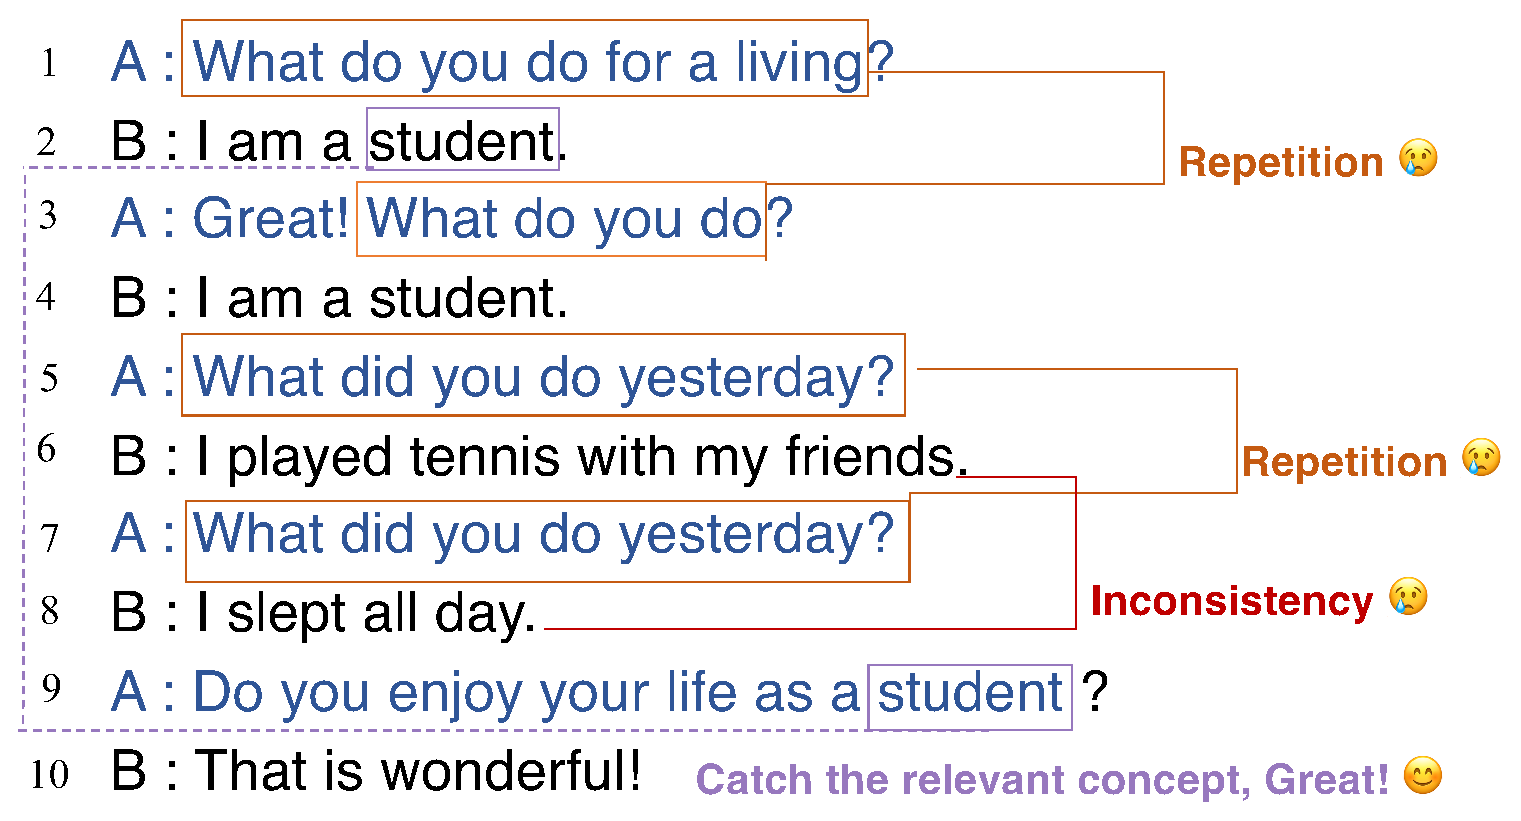
\includegraphics[width=0.95\columnwidth]{example2.eps}
        \caption{A chat snippet between two bots.}
        \label{fig:example}
\end{figure}

Fluency, Knowledge, Proactivity and Specificity are scored for each turn separately
and aggregated at the end of the conversation.
Detection for diversity, consistency and relevance are more involved and are explained
using \figref{fig:example}. 

As for diversity, at each turn $t$, we first check if there exists any repetitive question.  
We can easily find turn 3 and turn 7 repeated turn 1 and turn 5 
respectively. They will then be penalized one point for repetition. 
Repetition is not penalized if the previous turn is already 
marked as a repetitive question. For example, in \figref{fig:example}, 
although turn 4 is considered a repetition of turn 2,  
we are not going to penalize it as turn 3 is a repetitive question. 

The detection of inconsistency is always triggered after the detection of repeated questions. 
If the answers to the same questions are different, we will penalize the current turn, 
such as turn 8 in \figref{fig:example}.

We decide a repetition or an inconsistency by calculating the similarity of the two turns. 
We use a similarity function to complete the calculations, which we will 
discuss in \secref{sec:experiment}. The actual diversity and consistency scores
are the negation from the amount of repetition and inconsistency.

Relevance is assessed as a bonus to reward
a bot if it is able to memorize the important relevant concepts that have shown up 
before in the conversation. We sort the concepts that have shown up in 
chat history by their IDF scores. For example, in turn 9, $A$ 
mentions the concept word ``student'' presented by $B$ in turn 2. With this
turn, $A$ will win a bonus point.


The algorithms and notations for computing diviersty, consistency and relevance are included
in \tabref{tab:functions}, \algoref{algo:rep}, \algoref{algo:inconsist}, and \algoref{algo:bonus}. 

\begin{table}[th]
\centering
\small
\begin{tabular}{c|l}
%\hline
\toprule
\textbf{Notation} & \textbf{Description} \\ \midrule
$t$ & Current turn \\
$H(t)$  &  a list of history turns prior to $t$ \\
$Sim(x,y)$ & similarity between two turns $x$ and $y$ \\
$\sigma_r$ & Threshold for detecting repetition \\
$\sigma_c$ & Threshold for detecting consistency \\
$r$ & Weight for repetition \\
$c$ & Weight for inconsistency \\
$b$ & Weight for bonus \\
$d$ & Min distance between consecutive mentions \\
IDF list & List of lemma in chatlog sorted by IDF\\
$p$ & Percentage of important lemmas in IDF list\\
$R(t)$ &  Repetition penalty for turn $t$ \\
$C(t)$ &  Inconsistency penalty for turn $t$ \\ 
$B(t)$ &  Memory bonus for turn $t$ \\
$Rep(t)$ & A list of repeated turns for turn $t$ \\  
\bottomrule
\end{tabular}
\caption{
Functions and variables in algorithms.}
\label{tab:functions}
\end{table}

\begin{algorithm}[th]
\small
\caption{Scoring for Diversity}
\label{algo:rep}
\hspace*{0.02in} {\bf Input:}
 $t$, $H$, $Sim$, $\sigma_{r}$
; \hspace*{0.02in} {\bf Output: } 
 $R$;
\begin{algorithmic}[1]
\State //Starting to detect repetition
\For {$u$ in $H(t)$}
	\If {$Sim(t,u) \geq \sigma_{r}$}
		\State Add $u$ to $Rep(t)$
	\EndIf
\EndFor
    \If{$len(Rep(t))\geq 0$}
        \If{$t$ is a question and We can find a question in $Rep(t)$}
        \State $ R(t) \leftarrow  R(t) + 1$ 
        \Else
        \If {the previous turn of $t$ is not a repetitive question}
        \State $R(t)) \leftarrow R(t) + 1$ 
        \EndIf
        \EndIf
    \EndIf
\end{algorithmic}
\end{algorithm}


\begin{algorithm}[th]
\small
\caption{Scoring for Consistency}
\label{algo:inconsist}
\hspace*{0.02in} {\bf Input:}
$t$, $H$, $Sim$, $\sigma_{c}$
; \hspace*{0.02in} {\bf Output:  } 
 $C$;
\begin{algorithmic}[1]
\State // Inconsistency detection
 \If {previous turn of $p$ is a repetitive question} 
   \If{ the response $res$ to the question repeated by turn $p$ contradicts turn $i$ with $Sim(t, res) \leq \sigma_{c}$ }
    \State $C(t) \leftarrow C(t) + 1$
   \EndIf
  \EndIf
\end{algorithmic}
\end{algorithm}

\begin{algorithm}[th]
\small
\caption{Scoring for Relevance}
\label{algo:bonus}
\hspace*{0.02in} {\bf Input:}
$t$, $p$, $d$
; \hspace*{0.02in} {\bf Output:  } 
$B$;
\begin{algorithmic}[1]
\State // Assessing the ability of catching relevant concepts\\
$B(t) \leftarrow 0$
\For {all tokens $tk$ in current turn $t$}
 \If {$t$ - previous occurrence turn of $tk > d$ and $tk$ in the top $p\%$ of the IDF list of all tokens in the dialogue} 
   \State $B(t) \leftarrow 1$
  \EndIf
 \EndFor
\end{algorithmic}
\end{algorithm}

At the end of each game, each bot gets seven scores, one for each dimension.  
After pairwise comparison on individual dimension, a bot gains one point for win and zero point for a tie or lose.
The final score of each bot is determined by the sum of their individual scores.
%\KZ{Are these scores positive or negative? Comparable between bots?}

\subsubsection*{Match-level Scoring}
%\KZ{Use an equation to compute the final scores?}
One match which consists of two games, each started with a different bot, 
decides winning or losing between two bots.
For match-level scoring, we mimic the scoring rules of soccer tournament. 
For each match, $W$ points for the winner,  
$T$ points for a tie and 
$L$ points for the loser.
The value of $W$, $T$ and $L$ will be discussed in \secref{sec:ablation}. 

%\KZ{At the match level, we need to consider different starting context for the bots? I think we should present a few options for the reader and say that we are limited to these.}

\subsubsection*{Tournament-level Scoring}
%\KZ{Use an equation to compute the final scores?}
We count the points by simply summing up their scores gained in every match. Currently, several bots with the same final rank are tolerated. For future study, it's possible to mimic more detailed rules presented in sports match such as determine their ranking based on their win-loss relationship in the match between them.  
If they are still tied, we could propose an “overtime” for these two bots, one human judge may observe their performance and then make the decision of the game.

\section{Syntax of OCR Description Language}
\label{sec:syntax}

In this section, we introduce the OCR description language,
and explain what kind of structured data that ODL is able to describe.
The abstract syntax of ODL is formally described in \figref{fig:syntax}.
ODL is able to describe both structured data and
spatial layouts of textual information within the medical image.
In the following parts, we will discuss the ODL syntax and its type system in more detail.
% \newsavebox{\absfalign}
% \begin{lrbox}{\absfalign}
% % \fontsize{6pt}{7pt}\selectfont
% \begin{align*}
% \text{int} ::= ~&[-+]?[0-9]+ \\
% \text{float} ::= ~&[-+]?[0-9]*.[0-9]+ \\
% \text{num} ::= ~&int|float\\
% \text{len} ::= ~&num ~~ (pixel|cm) \\
% \text{coord} ::= ~&\langle len_1, ~~ len_2, ~~ len_3, ~~ len_4\rangle \\
% \text{bop} ::= ~&+|-|*|/|=|!=|<|>|<=|>=\\
% % \text{datatype} ::= 
% % ~&Oint(int, int)\\
% % |~& Ofloat(int, int, int, int)\\
% % |~& Ostring(string)\\
% \text{Value v} ::= 
% ~&() \\
% |~& int \\
% |~& float \\
% |~& string \\
% |~& len \\
% |~& coord \\
% % |~& {v_1, ~~ ..., ~ v_n}\\
% %|~& \{v_1 | v_2 | ... | v_n\}\\
% |~& \{v_1, ..., v_n\} \\
% \end{align*}
% \end{lrbox}

% \newsavebox{\abssalign}
% \begin{lrbox}{\abssalign}
% % \fontsize{6pt}{7pt}\selectfont
% \begin{align*}
% \text{Expression e} ::= 
% % |~& datatype ~~ x \tag{variable}\label{syntax:variable}\\
% ~&c \tag{constant}\label{syntax:constant}\\
% |~& x \tag{name}\label{syntax:name}\\
% % |~& nop ~~ e\\
% |~& e_0(e_1, e_2, ..., e_n) \tag{constraints} \label{syntax:constraints}\\
% % |~& \lambda x.e \tag{funciton}\label{syntax:function}\\
% % |~& e_1 ~~ e_2 \tag{apply}\label{syntax:apple}\\
% |~& hskip ~~e \tag{horizontal skip}\label{syntax:hskip}\\
% |~& vskip ~~e \tag{vertical skip}\label{syntax:vskip}\\
% |~& \{e_1 | e_2 | ... | e_n\} \tag{union}\label{syntax:union}\\
% % |~& \{e_1, ~~ ..., ~~ e_n\}\\
% % |~& e.i\\
% |~& \{e_1, ..., e_n\} \tag{struct}\label{syntax:struct}\\
% |~& e ~~ list \tag{list}\label{syntax:list}\\
% % |~& e_1[e_2] \tag{list element}\label{syntax:listele}\\
% |~& e ~~ as ~~ x \tag{blinding}\label{syntax:blinding}\\
% |~& e_1 ~~ bop ~~ e_2 \tag{binary operation}\label{syntax:bop}\\
% \end{align*}
% \end{lrbox}

% \begin{figure}[h]
% % \centering
% % \subfloat{\parbox{0.5\textwidth}{
% % {\usebox\absfalign}
% \begin{align*}
% \text{int} ::= ~&[-+]?[0-9]+ \\
% \text{float} ::= ~&[-+]?[0-9]*.[0-9]+ \\
% \text{num} ::= ~&int|float\\
% \text{len} ::= ~&num ~~ (pixel|cm) \\
% \text{coor} ::= ~&\langle len_1, ~~ len_2, ~~len_3, ~~ len_4\rangle \\
% \text{bop} ::= 
% ~&+|-|*|/\\
% |~& =|!=\\
% |~& <|>|<=|>=\\
% % \text{datatype} ::= 
% % ~&Oint(int, int)\\
% % |~& Ofloat(int, int, int, int)\\
% % |~& Ostring(string)\\
% \text{v} ::= 
% ~&() \\
% |~& int \\
% |~& float \\
% |~& string \\
% |~& len \\
% |~& coor \\
% % |~& {v_1, ~~ ..., ~ v_n}\\
% %|~& \{v_1 | v_2 | ... | v_n\}\\
% |~& \{v_1, ..., v_n\} \\
% % a = b\\
% % \end{align*}
% % }}
% % \end{subfloat}
% % \hfill
% % \subfloat{
% % \subfloat{\parbox{0.5\textwidth}{
% % {\usebox\abssalign}
% % \begin{align*}
% \text{e} ::= 
% % |~& datatype ~~ x \tag{variable}\label{syntax:variable}\\
% ~&c \tag{constant}\label{syntax:constant}\\
% |~& x \tag{name}\label{syntax:name}\\
% % |~& nop ~~ e\\
% |~& e_0(e_1, e_2, ..., e_n) \tag{constraints} \label{syntax:constraints}\\
% % |~& \lambda x.e \tag{funciton}\label{syntax:function}\\
% % |~& e_1 ~~ e_2 \tag{apply}\label{syntax:apple}\\
% |~& hskip ~~e \tag{horizontal skip}\label{syntax:hskip}\\
% |~& vskip ~~e \tag{vertical skip}\label{syntax:vskip}\\
% |~& \{e_1 | e_2 | ... | e_n\} \tag{union}\label{syntax:union}\\
% % |~& \{e_1, ~~ ..., ~~ e_n\}\\
% % |~& e.i\\
% |~& \{e_1, ..., e_n\} \tag{struct}\label{syntax:struct}\\
% |~& e ~~ list \tag{list}\label{syntax:list}\\
% % |~& e_1[e_2] \tag{list element}\label{syntax:listele}\\
% |~& e ~~ as ~~ x \tag{blinding}\label{syntax:blinding}\\
% |~& e_1 ~~ bop ~~ e_2 \tag{binary operation}\label{syntax:bop}\\
% % c = d\\
% % \text{Expression e} ::= 
% % % |~& datatype ~~ x \tag{variable}\label{syntax:variable}\\
% % ~&c\\
% % |~& x\\
% % % |~& nop ~~ e\\
% % |~& e_0(e_1, e_2, ..., e_n)\\
% % % |~& \lambda x.e \tag{funciton}\label{syntax:function}\\
% % % |~& e_1 ~~ e_2 \tag{apply}\label{syntax:apple}\\
% % |~& hskip ~~e\\
% % |~& vskip ~~e\\
% % |~& \{e_1 | e_2 | ... | e_n\}\\
% % % |~& \{e_1, ~~ ..., ~~ e_n\}\\
% % % |~& e.i\\
% % |~& \{e_1, ..., e_n\}\\
% % |~& e ~~ list\\
% % % |~& e_1[e_2] \tag{list element}\label{syntax:listele}\\
% % |~& e ~~ as ~~ x\\
% % |~& e_1 ~~ bop ~~ e_2\\
% \end{align*}
% % }}
% % \end{subfloat}
% \caption{Syntax}
% \label{fig:syntax}
% \end{figure}

\begin{figure}[h]
\small
\begin{align*}
\text{int} ::=~& \land-?\backslash d+\$\\
\text{float} ::=~& \land(-?\backslash d+)(.\backslash d+)?\$\\
\text{num} ::=~& int|float\\
\text{len} ::=~& num ~~ (pixel|cm)\\
\text{coor} ::=~& \langle len_1, len_2, len_3, len_4\rangle\\
\text{bop} ::= 
~& +|-|*|/\\
|~&=|!=\\
|~&<|>|<=|>=\\
% \text{datatype} ::= 
% ~&Oint(int, int)\\
% |~& Ofloat(int, int, int, int)\\
% |~& Ostring(string)\\
\text{v} ::=~& 
() \\
|~& int \\
|~& float \\
|~& string \\
|~& len \\
|~& coor \\
% |~& {v_1, ~~ ..., ~ v_n}\\
%|~& \{v_1 | v_2 | ... | v_n\}\\
|~& \{v_1, ..., v_n\} \\
%\end{align*}
%\begin{align*}
\text{e} ::= 
% |~& datatype ~~ x \tag{variable}\label{syntax:variable}\\
~& c \tag{constant}\label{syntax:constant}\\
|~& x \tag{name}\label{syntax:name}\\
% |~& nop ~~ e\\
|~& e_0(e_1, e_2, ..., e_n) \tag{constraints} \label{syntax:constraints}\\
% |~& \lambda x.e \tag{funciton}\label{syntax:function}\\
% |~& e_1 ~~ e_2 \tag{apply}\label{syntax:apple}\\
|~& hskip ~~e \tag{horizontal skip}\label{syntax:hskip}\\
|~& vskip ~~e \tag{vertical skip}\label{syntax:vskip}\\
|~& \{e_1 | e_2 | ... | e_n\} \tag{union}\label{syntax:union}\\
% |~& \{e_1, ~~ ..., ~~ e_n\}\\
% |~& e.i\\
|~& \{e_1, ..., e_n\} \tag{struct}\label{syntax:struct}\\
|~& e ~~ list \tag{list}\label{syntax:list}\\
% |~& e_1[e_2] \tag{list element}\label{syntax:listele}\\
|~& e ~~ as ~~ x \tag{blinding}\label{syntax:blinding}\\
|~& e_1 ~~ bop ~~ e_2 \tag{binary operation}\label{syntax:bop}\\
\end{align*}
\caption{Syntax}
\label{fig:syntax}
\end{figure}

\begin{figure}
\small
\begin{align*}
\text{t}::=~&unit\\
|~&int\\
|~&float\\
|~&len\\
%\end{align*}
%\begin{align*}
|~&\langle len, ~~ len, ~~ len, ~~ len\rangle\\
% &|~&t_1 \rightarrow t_2\\
|~&\{t_1 + t_2 + ... + t_n\}\\
|~&\{l_1 : t_1, ~~ ..., ~~ l_n : t_n\}\\
|~&t ~~ list\\
\end{align*}
\caption{ODL Data Types}\label{fig:type}
\end{figure}





% \KZ{Make \figref{fig:syntax} double column and more compact.}



\subsection{Primitive Expressions}
According to the abstract syntax, we start from the most primitive expressions
that ODL can describe: \textit{constant} and \textit{variable}.
Constants represent fixed-valued strings or numerical values to be recognized from the image.
For example in \figref{fig:running-odl-abstract}, ``Vent. rate'' and ``mm/mV''
are constant expressions, as they always occur in all ECGs of the same format.
% Constants are usually markers or delimiters in semi-structured data formats.
On the other hand, primitive variables represent numerical (int or float) values
varied in different images.
In \figref{fig:running-odl-abstract}, the variable $vr$ represents the
numerical value of ``Vent. rate''.%, which varies by different patients.
%Variables usually have a numeric type (int or float),
%and sometimes users know the constraints of its data field.
It's worth mentioning that,
the reason we specially define constants in ODL is to
enrich the relative layout information between different expressions,
so that the parser can locate the variables in the image more accurately.

\subsection{Spatial Expressions}
Spatial description expressions include \textit{hskip len} and \textit{vskip len}.
% These two expressions explicitly encode horizontal and vertical
% spacing information in the images, and we mainly explain the former one.
As shown in \figref{fig:running-ecg}, there has a large horizontal margin
between ``Vent. rate'' and ``63 bpm'', hence we can use \textit{hskip len} to
explicitly and approximately describe such horizontal margin
between the previous and next expressions.
% we can explain why needed here, because not all places have hskip/vskip.
The size of margin is determined by $len$, which has two parts:
the length value and its measurement unit.
Units can be the absolute pixel, or what are more encouraged,
the percentage of width ($w$) or height ($h$) of the image.
Besides, \textbackslash t stands for a special margin size,
which equals to the average width of 4 Latin characters.
We can easily estimate this value via the width of each text box
in the raw OCR results.
Similarly, \textit{vskip len} explicitly describes the vertical margin
between expressions, and \textbackslash n stands for the average height
of one Latin character.

\subsection{Composition}
Compositions are compound expressions constructed from other expressions.
These include \textit{union}, \textit{struct}, \textit{list}, \textit{binding}, \textit{bop} and \textit{constraint}.

The first three compositions define more structured and
complex type expressions.
The \textit{union} expression means there exists
multiple potential data or spatial expressions.
For example, the union description of $month\_str$ is the enumeration
of all abbreviations of different months.
The \textit{struct} expression is used to describe
an expression with multiple sub-expressions.
All sub-expressions must be described sequentially,
following the left-to-right then top-to-bottom manner.
As another example in \figref{fig:running-odl-surface},
the struct description of $triple\_t$ contains
the constant attribute name, spacing,
variable value and constant unit listed from left to right.
The \textit{list} expression indicates that a sequence of similar data or
the same spatial expressions should be applied multiple times.
In the example, \textit{vskip \textbackslash n list} represents several
blank lines between the data of interpretation and parameters in the images.

The function of \textit{binding} is to give a variable name \textit{x} to
the composition expression \textit{e}, so that each expression has an identifier
in the output parsing tree.
The function of \textit{bop} supports basic binary operations between numerical
values in the ODL.
These two expressions are designed to simplify the description of ODL.

Finally, the \textit{constraint} expression in ODL consists of two categories:
value constraints and spatial constraints.
Value constraints can be applied to the primitive variable,
indicating its type and value range, if the user knows in prior.
Since variables are usually numerical, two value constraints are available:
$x(int, v_{min}, v_{max})$ and
$x(float, length, precision, v_{min}, v_{max})$.
For example in \figref{fig:running-odl-abstract},
$day(int, 1, 31)$ constrains the variable to be an integer ranging from 1 to 31;
$p2(float, 3, 1)$ constrains the variable to be a floating number in length 3
and precision 1, without range limits.
Spatial constraints have the form $e(coor)$,
which can be applied to any expression,
and restrict the areas that corresponding data resides in the image.
Such positions in ODL are represented by $coor$, the 4-tuple of
left, top, right, bottom coordinates.
As shown in \figref{fig:running-odl-abstract}, spatial constraints
are applied to several structs: $time$, $tri$ and $inter$.
These constraints are rather rough and large,
as users are encouraged to give larger spatial constraints
if they are not so sure of the exact bounding boxes.


\subsection{Type System}

% In ODL, we can assign a types to every expression.
% We set up some rules determining types for expressions,
% which make up a complete type system.
The inductive typing rules of ODL is shown in \figref{fig:typingrule}.
% The type system of ODL is shown in \figref{fig:type} and \figref{fig:typingrule}.
% \figref{fig:type} shows the basic principles for determining types and
% \figref{fig:typingrule} extends it by providing inductive typing rules.
\textit{T-VARIABLE} indicates that the type of \textit{variable} is
based on the type of name in the typing context.
\textit{T-INT ARITH}, \textit{T-INT REL}, \textit{T-FLOAT ARITH} and
\textit{T-FLOAT REL} indicate that the two expressions of the \textit{bop}
are of the same type (int or float), and the final type of the \textit{bop}
expression is based on the binary operation.
\textit{T-CONSTRAINT} indicates that the final type of the \textit{constraints} expression is always the same as the original expression $e_0$.
\textit{T-HSKIP} and \textit{T-VSKIP} indicate that the spatial parameter $e$
is of the \textit{len} type, and the final types of these two expressions
should be \textit{unit}.
The last three of the typing rules are for
the \textit{union}, \textit{struct} and \textit{list} expressions, respectively.

% \begin{figure}[ht]
% % \centering
% \begin{minipage}{0.4\columnwidth}
% \begin{align*}
% \text{t}::=~&unit\\
% |~&int\\
% |~&float\\
% |~&len\\
% \end{align*}
% \end{minipage}
% \begin{minipage}{0.4\columnwidth}
% \begin{align*}
% |~&\langle len, ~~ len, ~~ len, ~~ len\rangle\\
% % &|~&t_1 \rightarrow t_2\\
% |~&t_1 + ... + t_n\\
% |~&t_1 * ... * t_n\\
% |~&t ~~ list\\
% \end{align*}
% \end{minipage}
% \caption{ODL Data Types}\label{fig:type}
% \end{figure}

\begin{figure}[ht]
% \centering
\begin{align*}
  \tag{T-VARIABLE}
  &\frac
  {\Gamma(x)=t}
  {\Gamma \vdash x:t}\\
  \tag{T-INT ARITH}
  &\frac
  {\Gamma \vdash e_1:int ~~ \Gamma \vdash e_2:int ~~ bop \in \{+,-,*,/,\%\}}
  % bop \in \{+,-,*,/,\%, =, !=, >, <, <=, >=\}
  {\Gamma \vdash e_1 ~~ bop ~~ e_2 :int} \\
  \tag{T-INT REL}
  &\frac
  {\Gamma \vdash e_1:int ~~ \Gamma \vdash e_2:int ~~ bop \in \{=, !=, <, >, <=, >=\}}
  % bop \in \{+,-,*,/,\%, =, !=, >, <, <=, >=\}
  {\Gamma \vdash e_1 ~~ bop ~~ e_2 :bool} \\
  \tag{T-FLOAT ARITH}
  &\frac
  {\Gamma \vdash e_1:float ~~ \Gamma \vdash e_2:float ~~ bop \in \{+,-,*,/,\%\}}
  % bop \in \{+,-,*,/,\%, =, !=, >, <, <=, >=\}
  {\Gamma \vdash e_1 ~~ bop ~~ e_2 :float}\\
  \tag{T-FLOAT REL}
  &\frac
  {\Gamma \vdash e_1:float ~~ \Gamma \vdash e_2:float ~~ bop \in \{=, !=, <, >, <=, >=\}}
  % bop \in \{+,-,*,/,\%, =, !=, >, <, <=, >=\}
  {\Gamma \vdash e_1 ~~ bop ~~ e_2 :bool}\\
  \tag{T-CONSTRAINT}
  &\frac
  {\Gamma \vdash e_0:t_0, \Gamma \vdash e_1:t_1, ..., \Gamma \vdash e_n:t_n}
  {\Gamma \vdash e_0(e_1, e_2, ..., e_n):t_0}\\
  % \tag{T-FUNCTION}
  % &\frac
  % {\Gamma[x:t_1] \vdash e:t_2}
  % {\Gamma \vdash fn ~~ x=> e:t_1 \rightarrow t_2} \\
  \tag{T-HSKIP}
  &\frac
  {\Gamma \vdash e:len}
  {\Gamma \vdash hskip ~~ e:unit}\\
  \tag{T-VSKIP}
  &\frac
  {\Gamma \vdash e:len}
  {\Gamma \vdash vskip ~~ e:unit}\\
  \tag{T-UNION}
  &\frac
  {for ~~ each ~~ i ~~ \Gamma \vdash e_i:t_i }
  {\Gamma \vdash \{e_1|...|e_n\}:t_1+...+t_n}\\
  \tag{T-STRUCT}
  &\frac
  {for ~~ each ~~ i ~~ \Gamma \vdash e_i:t_i }
  {\Gamma \vdash \{e_1, ..., e_n\}:t_1*...*t_n}\\
  % \tag{T-UNION}
  % &\frac
  % {for ~~ each ~~ i ~~ \Gamma \vdash e_i:t_i }
  % {\Gamma \vdash \{e_1|...|e_n\}:t_1+...+t_n}\\
  \tag{T-LIST}
  &\frac
  {\Gamma \vdash e:t}
  {\Gamma \vdash e~~list:t~~list}\\
  % \tag{T-LIST ELEMENT}
  % &\frac
  % {\Gamma \vdash e_1:t~~list ~~ \Gamma \vdash e_2:int}
  % {\Gamma \vdash e_1[e_2]:t}\\
\end{align*}
\caption{Inductive typing rules of ODL.}\label{fig:typingrule}
\end{figure}


% \textit{unit} type are for the
% expression of \textit{()} value. \textit{int}, \textit{float} and \textit{float} are types
% of the expressions that can be parsed into these type of values. \textit{len} is
% the type of \textit{len} value. The rest four kinds of types are the combination of
% all the types. \textit{$\langle len ~~ len, ~~ len, ~~ len\rangle$} is the type for
% \textit{coord}. \textit{$\{t_1 + t_2 + ... + t_n\}$} is the type for \textit{union} expression, which
% means the type of the value of \textit{union} can be any type of the components of the expression.
% \textit{$\{l_1 : t_1, ~~ ..., ~~ l_n : t_n\}$} is the type for \textit{struct}. All the types of
% the subexpressions in \textit{struct} are recorded. Finally, \textit{t ~~ list} is the type for
% \textit{list}. \textit{list} is made up of a sequence of the expressions in the same type.
% In \figref{fig:typingrule}, the detailed typing rules are described. Other than the types
% of the expressions, \textit{T-INT ARITH}, \textit{T-INT REL}, \textit{T-FLOAT ARITH} and \textit{T-FLOAT REL}
% indicate that the two expressions of the \textit{bop} shown be in the same type, int or float, and
% the final type of the \textit{bop} expression is based on the binary operation. \textit{T-CONSTRAINS}
% indicates that the types of the expressions in the constraints have nothing to do with the
% final type of the \textit{constraints} expression.

\section{Robust ODL Parser}
\label{sec:parsing}

In this section, we focus on the ODL parser,
which is the core of the entire information extraction system.
% we focus on the process of structured textual information extraction,
% which is the kernel part of the entire system.
We first describe the semantics that the parser is used for generating
parsing trees based on the ODL specification.
Afterwards, we describe the detail of the fuzzy matching strategy
and the automatic correction model.

\subsection{Semantics of the ODL Parser}
% 1. in general, what's the parsing process
Referring to \figref{fig:running-parsing-tree},
the parsing process evaluates the entire data expression of ODL
into hierarchical texts organized by the parsing tree,
defined as $T = (node, [T_1, ..., T_n])$,
where $T_i$ is the $i$-th sub-tree of $T$.
The leaf nodes of $T$ are $(e, text)$ pairs representing the alignment
between some primitive expression and its corresponding text,
and non-leaf nodes are always the variable names $x$.

% 2. recursive process
Since the entire expression has a complex structure,
the evaluation is conducted recursively:
it first evaluates each sub-expression, and then composes multiple parsing trees
into a large one.
So the semantics of the parser consists of two parts:
the evaluation rules for non-compositional expressions
(constants, primitive variables and spatial expressions),
and the inductive evaluation rules for compositional expressions.

% talk about basic
% \subsubsection{Evaluation Rules for Non-compositional Expressions}
The most basic rule is for evaluating constants (or primitive variables):
given the OCR data $D$ and the constant (or primitive variable) $e$ in ODL,
searching all possible alignments between $e$ and some text box $d \in D$.
During the whole parsing process, the parser maintains an environment
$E = (x_0, y_0, x_1, y_1, x_{cr}, y_{cr})$,
which contains the coordinates of the searching area,
as well as a cursor ($x_{cr}$, $y_{cr}$).
The cursor is a reference point, indicating the rough position
that the desired text box resides.
By default, the searching area is the whole image,
and the cursor is at the top-left corner.
The relative layout in ODL is represented in a
left-to-right then top-to-bottom manner,
thus the text box $d$ becomes a candidate alignment of $e$,
if it's within the searching area,
and not located in the top-left side of the cursor.
The following $InBound$ function defines such rule:
\begin{equation}
  \begin{aligned}
      InBound(D, E) & = \{d \in D\ |\ \\
      & E.x_0 \leq d.x_0 \leq d.x_1 \leq E.x_1 \\
      \land &
      E.y_0 \leq d.y_0 \leq d.y_1 \leq E.y_1 \\
      \land & \lnot
      ( d.x_1 \leq E.x_{cr} \land d.y_1 \leq E.y_{cr} )
      \}. \\
  \end{aligned}
\end{equation}
With the environment $E$ provided,
the parser enumerates all candidate text boxes,
and use a boolean match function $Match(e, d; E)$ to
judge whether an alignment exists between $d$ and
the constant (or primitive variable) $e$.
Intuitively, $d$ is a valid match of $e$,
if its text is close to the constraints of $e$,
and it's located near the cursor ($E.x_{cr}, E.y_{cr}$).
For a better flow of explanation, the formal definition of the match function
will be given in the next section.
If matches, a new parsing tree $T=((e, d.text), [])$ is generated,
which has a single node without any children.
Besides, both $D$ and $E$ need to be changed, so that the parser
can work on the alignment of the subsequent expressions in ODL.
Following the relative layout of expressions,
the cursor is moved to the top-right corner of the box:
$E' = Move(E, d)$, and $d$ is removed from $D$,
as one text box can be aligned at most once: $D' = D - \{d\}$.
\equref{equ:semantic-operations} defines a series of functions
that changes the environment, which are used in different evaluation rules.
In which, $c$ is short for $coor$.
\begin{equation}
  \begin{aligned}
    Move(E, d) = & (E.x_0, E.y_0, E.x_1, E.y_1, d.x_1, d.y_0), \\
    Hskip(E, len) = & (E.x_0, E.y_0, E.x_1, E.y_1, E.x_{cr}+len, E.y_{cr}), \\
    Vskip(E, len) = & (E.x_0, E.y_0, E.x_1, E.y_1, E.x_0, E.y_{cr}+len), \\
    Restrict(c) = & (c.x_0, c.y_0, c.x_1, c.y_1, c.x_0, c.y_0). \\
  \end{aligned}
  \label{equ:semantic-operations}
\end{equation}

The tuple $(T, E, D)$ is called a \textit{parsing state},
which records the partial parsing tree,
the environment information and the remaining text boxes.
Since there exist multiple candidate text boxes for alignment,
given $E$ and $D$, $e$ will be evaluated into a set of parsing states,
written in the following judgment form:
\begin{equation}
  E,D;e \Downarrow \bigcup_{i} \{(T_i, E'_i, D'_i)\}.
\end{equation}


\begin{figure*}[ht!]
% \[
%   {\rm Judgment~ Form:}~~ E,D;e \Downarrow (D';parse\_tree)list
%   \label{semantic:judegement}
% \]
% where E is environment, D and D' are input\_data, C records the position of the cursor.
\begin{gather*}
  \tag{\sc E-Empty}\label{rule:empty}
  \frac
  {InBound(D,E)=\emptyset}
  {E,D;e \Downarrow \{(((e, Nil), []), E, D)\}}\\
  \tag{\sc E-PRIM1}\label{rule:c1}
  \frac
  {d \in InBound(D,E), Match(e, d; E)=True, E'=Move(E, d) ~~ E',D-\{d\};e \Downarrow r}
  {E,D;e \Downarrow r \cup \{ (((e, d.text), []), E', D-\{d\} ) \} }\\
  \tag{\sc E-PRIM2}\label{rule:c2}
  \frac
  {d \in InBound(D,E), Match(e, d; E)=False, E'=Move(E, d) ~~ E',D-\{d\};e \Downarrow r}
  {E,D;e \Downarrow r \cup \{ (((e, Nil), []), E', D-\{d\} ) \} }\\
  \tag{\sc E-Hskip}\label{rule:hskip}
  \frac
  {E'=Hskip(E,len)}
  {E,D;hskip\ len \Downarrow \{(Nil,E',D)\}   }\\
  \tag{\sc E-Vskip}\label{rule:vskip}
  \frac
  {E'=Vskip(E,len)}
  {E,D;vskip\ len \Downarrow \{(Nil,E',D)\}   }\\
  \tag{\sc E-Coor}\label{rule:coor}
  \frac
  {E'=Restrict(coor), D'=InBound(D,E') ~~ E',D';e \Downarrow \bigcup_{i} \{(T_i, E''_i, D''_i)\}}
  {E,D;e(coor) \Downarrow \bigcup_{i} \{(T_i, (E.x_0, E.y_0, E.x_1, E.y_1, E''_i.x_{cr}, E''_i.y_{cr}), D-D'+D''_i)\}}\\
  \tag{\sc E-Wrap1}\label{rule:wrap1}
  \frac
  {E,D;e \Downarrow \bigcup_i \{(T_i, E'_i, D'_i)\}}
  {E,D;\{e\}\ as\ x \Downarrow \bigcup_i \{((x, [T_i]), E'_i, D'_i)\}} \\
  \tag{\sc E-Wrap2}\label{rule:wrap2}
  \frac
  {E,D;e \Downarrow \bigcup_i \{(T_i, E'_i, D'_i)\}}
  {E,D;e\ list\ as\ x \Downarrow \bigcup_i \{((x, [T_i]), E'_i, D'_i)\}} \\
  \tag{\sc E-Union}\label{rule:union}
  \frac
  {E,D;\{e_1\}\ as\ x \Downarrow r_1 ~~ E,D;\{e_2|..|e_n\}\ as\ x \Downarrow r_2}
  {E,D;\{e_1|e_2|...|e_n\}\ as\ x \Downarrow r_1 \cup r_2}\\
  \tag{\sc E-Struct}\label{rule:struct}
  \frac
  {E,D;e_1 \Downarrow \bigcup_i \{(T_i, E'_i, D'_i)\} ~~
  \forall i: E'_i,D'_i;\{e_2,...,e_n\}\ as\ x \Downarrow
  \bigcup_j \{((x, [T_{2ij},...,T_{nij}]), E''_{ij}, D''_{ij})\}}
  {E,D;\{e_1,e_2,...e_n\}\ as\ x \Downarrow
  \bigcup_{ij} \{((x, [T_i, T_{2ij},...,T_{nij}]), E''_{ij}, D''_{ij})\}}\\  \tag{\sc E-List}\label{rule:list}
  \frac
  {E,D;e_1 \Downarrow \bigcup_i \{(T_i, E'_i, D'_i)\} ~~
  \forall i: E'_i,D'_i;e\ list\ as\ x \Downarrow
  \bigcup_j \{((x, \textbf{\textit{T}}_{ij}^{(child)}), E''_{ij}, D''_{ij})\}}
  {E,D;e\ list\ as\ x \Downarrow
  \bigcup_{ij} \{((x, [T_i] + \textbf{\textit{T}}_{ij}^{(child)}), E''_{ij}, D''_{ij})\}}\\
  % \tag{\sc E-List}\label{rule:list}
  % \frac
  % {E,D;e \Downarrow (E',D';parse\_tree)list ~~~~ }
  % {E,D;e ~~ list \Downarrow }\\
\end{gather*}
\caption{Evaluation rules of the ODL parser.}
\label{fig:semantics-kangqi}
\end{figure*}


% give rules for basic
Based on the definition of the environment, match function and parsing state,
\figref{fig:semantics-kangqi} lists all the evaluation rules.
The rules \ref{rule:empty}, \ref{rule:c1} and \ref{rule:c2} are used for
evaluating the constants or primitive variables in a recursive form,
where $r$ stands for a list of parsing states.
The parser generates new parsing trees based on whether $d$ and $e$ matches.
In addition, the parser can simply skip the text box $d$ and try to find
alignments from remaining OCR data $D-\{d\}$.

The rules \ref{rule:hskip} and \ref{rule:vskip}
are used for evaluating the spatial expressions.
Intuitively, the $hskip$ and $vskip$ expression doesn't match any text boxes,
but indicating the rough size of spacings.
Therefore, both rules merely move the cursor horizontally or vertically,
using $Hskip$ or $Vskip$ function defined in \equref{equ:semantic-operations}.

% talk about compositional
Now we introduce the evaluation rules for compositional expressions,
and focus on how the output parsing states are composed from
the multiple sub-states.
The rule \ref{rule:coor} is used for evaluating spatial constraints $e(coor)$.
The given coordinates $coor$ restrict the searching area of alignments
in the image, thus both the environment and the available OCR data are modified
when evaluating $e$.
The $Restrict$ function sets the new environment based on $coor$,
and the OCR data in the output parsing state contains
all text boxes outside the searching area ($D-D'$),
as well as unused boxes inside it ($D''_i$).
There doesn't have a evaluation rule for value constraints,
but such constraints will be used in the match function.

The last 5 rules in \figref{fig:semantics-kangqi} are used for evaluating
\textit{union}, \textit{struct} and \textit{list} expressions.
The rules \ref{rule:wrap1} and \ref{rule:wrap2}
construct the hierarchical structure of parsing trees,
where the root node $x$ is the identifier of union/struct/list expressions;
\ref{rule:union} simply combines parsing states from all its branches;
\ref{rule:struct} binds the parsing tree of $e_1$ to the larger tree of
the remaining parts;
\ref{rule:list} is similar with \ref{rule:struct}, considering that
a list equals to a struct with unlimited expressions.



\subsection{Fuzzy Match Function}
% 1. the parser works fuzzily.. (emmm)
% 2. two meanings: data: allows inexact match (15o, vcnt rule)
%                  spatial: not assigned precise boundary to every c/v
% 3. To tolerate the errors and noises,
%    we define functions measuring the distance of matching
%    at both data and spatial level, named xxx and yyy.
% 4. Match function are built based on them.
The key feature of the parsing process is the robustness:
rather than conducting exact match,
the parser tolerates the OCR recognition errors,
and the slight layout variances between images of the same format.
In order to measure the degree of fuzzy matching
between primitive expressions and text boxes,
we define penalty functions at both value and spatial level,
then based on that, we give the formal definition of the $Match$ function.
% We first discuss
% the parser can align under inexact match,
% with no precise boundary.
% Instead, using a fuzzy match function, which consider
% both data and spatial fitness between text box and expressions.
% We discuss these two points, and then give a formal definition of match function.
% Due to the limitations of OCR techniques, data derived from images is not 100\%
% correct. To tolerate the errors and noises in the OCR results, a scoring
% policy is proposed to take consideration of the constraints and OCR results.


\paragraph{Penalty Function for Value Constraints}
The value penalty function $F_v(e, text)$ measures the penalty of
aligning some text with the primitive expression $e$,
i.e., either constants or primitive variables.
For the constant $c$, since the desired value is fixed, the penalty score
is simply derived from the edit distance (Levenshtein distance)
between two texts,
which measures the minimal number of edits required to change one text to
the other.
For the primitive variable $x$ of the integer and floating point type,
the value constraint is put into use.
Referring to the value constraints $x(int, v_{min}, v_{max})$ and
$x(float, length, precision, v_{min}, v_{max})$,
edit distances are calculated between the text data and each numerical value,
satisfying the restrictions of value range, length or precision,
and the smallest edit distance is picked as the error score.
The complete form of the value penalty $F_v(e, text)$ is defined as follows:

\begin{equation}
  \begin{aligned}
    F_v(& c,text) = EditDist(c, text), \\
    F_v(& x(int,v_{min},v_{max}),text)= \min_i\{ \\
        & EditDist(i,text)\ |\ i \in Z, v_{min} \leq i \leq v_{max}\}, \\
    F_v(& x(float,l,p,v_{min},v_{max}),text)= \min_i\{ \\
        & EditDist(i,text)\ |\ i \in R', v_{min} \leq i \leq v_{max}\}, \\
  \end{aligned}
\end{equation}

\noindent
where $R'$ is the set of all real numbers in length $l$ and precision $p$.
For example, the penalty score (edit distance)
between the \textit{constant} ``Vent. rate'' and the text ``Vcnt. rule'' is 3.
As another example, the penalty score between $x(int, 60, 100)$ the text ``53''
is 1, since for all desired integers between 60 and 100,
``63'' holds the minimum edit distance with ``53'', which is 1.

\paragraph{Penalty Function for Spatial Layout}
Recap that in the parsing process, based on the left-to-right and top-to-bottom
relative layout between expressions embedded in ODL,
the cursor $(E.x_{cr}, E.y_{cr})$ maintains a rough reference position
that the desired text box resides.
That's to say, the closer a text box $d$ to the cursor,
the higher confidence to align with the current expression.
Therefore, the spatial penalty score $F_s(d, E)$ measures the spatial distance
between the cursor and the top-left corner of box, calculated in L$_1$-norm:
% TODO: unit in len / width.
\begin{equation}
	F_s(d, E) = |d.x_0 - E.x_{cr}| + |d.y_0 - E.y_{cr}|.
\end{equation}

Now we formally define the match function $Match(e, d; E)$.
The function returns a boolean value for whether the text box $d$
can be aligned to the primitive expression $e$.
Given the above penalty functions at both value and spatial view,
the $Match$ function is defined as the weighted sum of two scores,
controlled by an output threshold $\tau$:
\begin{equation}
Match(e, d; E) =
\begin{cases}
\text{T}& \text{$F_v(e, d.text)+k\cdot F_s(d, E) < \tau$}\\
\text{F}& \text{otherwise}
\end{cases}
.
\label{equ:match}
\end{equation}
\noindent
where $k$ and $\tau$ are hyperparameters of the system.
Finally, for picking the best parsing tree
from multiple parsing states of the entire image expression,
the textual error score of each primitive expression equally contributes
to the final score of the whole parsing tree $T$.
We define the overall score of $T$ as follows:
\begin{equation}
  score(T) = \sum_{(e,text) \in leaf(T)} F_v(e, text).
  \label{equ:overall}
\end{equation}


\subsection{Automatic Correction Module}
% 1. what's the correction model
The correction module aims at automatically detecting and correcting
error texts during the parsing process.
For example, the parser not only detects the error of matching the text ``15o''
to the variable $p1$ in \figref{fig:running-parsing-tree},
but also tries to correct the error text into ``150'' on-the-fly.
We first explain the automatic correction in the parsing process,
then discuss the incremental generation of the correction model.

% 2. formally define M, S
\subsubsection{Correction Model}
The correction model $M$ is a set of correction strategies $S$.
Each correction strategy $S$ is a probabilistic distribution of replacements
from the original string $ori$ to multiple candidate strings $dst$:
\begin{equation}
  S = \{(ori, dst_1, p_1), ..., (ori, dst_m, p_m)\}.
\end{equation}
\noindent
A concrete correction strategy, for example,
$S = \{(\text{``o''}, \text{``o''}, 0.6), (\text{``o''}, \text{``0''}, 0.3), (\text{``o''}, \text{``O''}, 0.1)\}$ indicates that given the character ``o''
there's a 60\% possibility that no correction is needed,
30\% possibility to replace into ``0'',
and another 10\% possibility to replace into ``O''.
Since the most frequent error of OCR recognition happens at character level,
all the original strings are short phrases (1,2,3-letter-gram).
In addition, we define $rep(text, ori, dst)$ as the result of
replacing all occurrences of $ori$ with $dst$ in the string $text$.

% 3. correction model-based scoring.
% define rep, es_with_prob, improved induction rule.
Given the correction model $M$,
the parser is able to vary the input text
such that a lower penalty for value constraints results.
Intuitively, the value penalty between ``15o'' and $x(int)$
is always 1 without correction.
It will become smaller than 1 when the correction model is applied,
due to a possibility of varying ``15o'' to ``150''.
More specifically, the relaxed version of value penalty $F'_v$
is the minimum expectation score of different texts
after being replaced by some strategy $S$:
\begin{equation}
\begin{aligned}
F'_v(e, text; M)=\min_{S \in M}\{ &
  \sum_{(dst_i, p_i) \in S} p_i \cdot F_v(e, text'_i)~ |~ \\
  & text'_i=rep(text, ori, dst_i)\}.
\end{aligned}
\end{equation}

By changing $F_v$ in \equref{equ:match} into $F'_v$,
the matching function $Match(e, d; E, M)$ is able to make better judgments
with the help of the correction model.
Once some $d$ and $e$ matches (\figref{fig:semantics-kangqi}, \ref{rule:c1}),
We record the best strategy $S^\star$ which reaches the minimum value penalty,
and generate the corresponding parsing tree $T_i = ((e, d.text'_i), [])$
for each variant of string replacement by $S^\star$.
For example, (p1, ``15o''), (p1, ``150'') and (p1, ``15O'')
are all valid parsing trees.
The best parsing result will be picked by the overall scoring function
defined in \equref{equ:overall}.
In this case, the system is able to find the correct matching results
from those candidate variants.


\subsubsection{Generation of Correction Model}
% 4. how the correction model is incrementally updated.
% what's the beginning,
The model is generated in a hybrid approach.
The initial correction model is generated from the result of OCR engine.
For each text box, the OCR engine outputs top-K candidate texts, although
only the best one is displayed in the raw OCR result.
Regarding each $i$-th candidate as the replacement of the best text,
the system counts all different ($ori$, $dst$) substring replacements.
For example, given the replacement from ``15o'' to ``150'',
distinct substring replacements are:
(``1'', ``1''), (``5'', ``5''), (``o'', ``0''),
(``15'', ``15''), (``5o'', ``50'') and (``15o'', ``150'').
For those images of the same format,
the system counts all occurrences of substring replacements from every image,
and builds the initial correction model $M$,
where the probabilities are calculated by normalization over occurrences.

The correction model can be updated by incremental human corrections.
Once the user manually changes some error texts into correct ones,
the system obtains new substring replacements ($ori$, $dst$)
and re-calculates all the probabilities in $M$.
Since the human labeled texts are ground truth texts,
all occurrences of substring replacements derived from human correction
are multiplied by a weight factor $w$,
so as to make larger contributions to the probability values in $M$.




% Model initiates by OCR software.
%
% Incremental learnt by human.
%
% Also: prompt users with most frequent error,
% associated with primitive / consts across multiple images.
%
% (random / frequent: leave to experimental settings)
%
% % \begin{enumerate}
% % \item incremental learning model, features;
% % \item How do we figure out which error should be corrected first;
% % \item What will happen after an error been corrected and
% % why the process is incremental.
% \label{sec:incremental}
% The correction model mentioned in \secref{sec:corrmodel}
% is an incremental learning model because
% the model is incrementally changed according to the corrections that
% humans make. The design of the correction model adheres to the scoring
% policy in \secref{sec:score}.
%
% \paragraph{Initial Model}
% % \KZ{Correct all the backquotes!}
% Before the results been corrected by human,
% the initial model is generated using the candidate results of the OCR
% engine. For example, for ``QRS'' in the example image, based on the OCR
% engine, the most reliable result is ``ORS''. Other top candidates are
% ``QPS'', ``QRS'' and ``OPS''. So we can learn from them that ``OR'' can be
% corrected as ``QP'', ``QR'' or ``OP''. These three candidates
% will be added into the initial model.
%
% To calculate the probabilities of the correction candidates in the initial
% model, we count the occurrence of each correction. In the example, the
% probabilities for ``OR'' corrected as ``OR'', ``QP'', ``QR'' or ``OP'' are equal
% since such corrections only happened once.
%
% % \[
% % P(newStr|oriStr) = \frac{occurrence ~of~ ()}{\sum_{tar \in all} occurrence ~of~ C(oriStr)=tar}
% % \]
%
% \paragraph{Training From Human Correction}
% After generating the parsing results using the initial model, we have
% made full use of the OCR engine. To correct the remaining errors,
% human input is needed. The incremental learning model is also suitable
% for learning from human correction.
%
% For example, if a human corrects the error result ``1o.o'' to ``10.0'',
% we can learn from it that for ``o''s in the OCR results, it's possible that
% they should be corrected as ``0''s. So the correction strategy
% for ``o'' is modified and ``0" is the new correct candidate.
% We also calculate the occurrence
% of different human correction for the probability calculation.
%
% \paragraph{Application of the Model}
% The model for correction is used in the scoring policy in the
% fuzzy parser. As shown in \secref{sec:score}, for each
% description, our system will consider all the potential
% results based on the correction strategies in the model.
% For the description ``QRS'' and the most confident results
% of OCR ``ORS'', we will try all the strategies in the model
% and consider both whether the corrected result satisfies the
% description and whether the correction strategy is
% feasible. In this example, since the four correction strategies
% are the same probability to happen, we choose ``QR'' as the correction
% result for ``OR'',
% which has the lowest error score based on the description.
%
% \subsubsection{Manual Correction Policy}
% In this section, we describe the policies for recommending
% errors to be manual corrected. When making use of human correction
% we find that some errors will have a greater impact on
% accuracy if they are corrected. The reason is some similar errors
% occur frequently. Which errors are recommended to a user
% for correction will affect the accuracy and the
% number of corrections that the user has to made.
%
% \paragraph{Random}
% The baseline for correction recommendation is random
% recommendation. Based on the parsing results, we can randomly
% recommend the errors we found for humans to correct.
%
% % \subsubsection*{Most Frequently Error Type}
%
% \paragraph{Most Frequent Error Description Elements}
% Another more efficient way to perform manual correction is to
% recommend the description
% elements that contain the most frequent errors. For a set of images
% in similar formats and the corresponding ODL descriptions,
% we find out which elements in the description are more likely
% to be parsed with errors. For those elements, similar errors
% are more likely to happen since the descriptions for them are the
% same. In this way, our recommendations can be more
% accurate than
% a random recommendation.

%
\section{Experiment}
In this section, we experiment on different NLG tasks. We first present the experimental setup on different tasks. Then, we show the quantitative and qualitative results together with comprehensive analysis and ablation studies.

\subsection{Implementation Details}
We evaluate the newly proposed ICL strategy on five commonly-researched natural language generation tasks: reading comprehension, dialogue summarization, style transfer, question generation and news summarization. Details on the task description, the strong baseline, corresponding  dataset, evaluation metrics and key hyper-parameters for each task are presented as follows.

\begin{table*}[th]
	\scriptsize
	\centering
	\begin{tabular}{lp{1.1cm}rrrcccc}
		\hline
		Task & Dataset & \#Train & \#Val & \#Test & Input & Output & Avg & Std\\
		\hline
		Reading Comprehension & DREAM & 6,116 & 2,040 & 2,041 & ``Q:''+ question + dialogue & answer & 5.59 & 2.61\\
		Dialogue Summarization & SAMSum & 14,732 & 818 & 819 & dialogue & summary  & 24.99 & 13.06\\
		Style Transfer & Shakespeare & 36,790 & 2,436 & 2,924 & original/modern  & modern/original  & 11.63 & 8.19 \\
		Question Generation & SQuAD1.1 & 75,722 & 10,570 & 11,877 & passage + [SEP] + answer & question & 13.09 & 4.27 \\
		News Summarization & CNNDM & 287,227& 13,368& 11,490 & document & summary & 70.97 & 29.59\\ 
		\hline
	\end{tabular}
	\caption{A summary of tasks and datasets. \#Train, \#Val and \#Test refers to the number of samples in the corresponding dataset. Avg and Std are the statistics for the number of output tokens. ``+'' refers to the concatenation operation.}
	\label{tab:taskdata}
\end{table*}

\textbf{Reading comprehension} is the task that answering questions about a piece of text. We use the DREAM dataset~\cite{sun2019dream} where questions are about corresponding dialogues and the answer is a complete sentence in natural language. We neglect the negative choices in the original dataset and formulate it as a NLG task. We adopt the pre-trained language model BART~\cite{lewis2020bart} as the baseline, where the input is a concatenation of a question and the corresponding dialogue made up of speakers and utterances. 
We experiment with  transformers\footnote{\url{https://github.com/huggingface/transformers}} based on the publically available ``facebook/bart-large'' checkpoint \footnote{\url{https://huggingface.co/facebook/bart-large}}.
%The preceding BART model is also adopted as the baseline, whereas the input is a concatenation of question and a dialogue.
The generated answers are evaluated by BLEU scores\footnote{The BLEU-1/2/3/4 scores are computed according the Google's implementation(\url{https://github.com/tensorflow/nmt/blob/master/nmt/scripts/bleu.py}).}~\cite{papineni2002bleu} widely used for QA systems, together with Meteor and Rouge-L F1 as mentioned above. The parameters are also the same as dialogue summarization, except that the early-stop is activated if there is no improvement on the perplexity of the validation set. 


\textbf{Dialogue summarization} is to generate a concise summary covering the salient information in the input dialogue. The preceding model BART has shown to be a strong baseline for this task, where only the dialogue is concatenated into a single sequence as the input. We experiment with  %transformers\footnote{\url{https://github.com/huggingface/transformers}} based on the publically available ``facebook/bart-large'' checkpoint \footnote{\url{https://huggingface.co/facebook/bart-large}} and 
SAMSum dataset\footnote{\url{https://arxiv.org/src/1911.12237v2/anc/corpus.7z}}~\cite{gliwa2019samsum} for daily-chat dialogues. 
The generated summaries are evaluated by comparing with the reference through evaluation metrics, including Rouge-1/2/L F1 scores\footnote{\url{https://github.com/pltrdy/files2rouge}}~\cite{lin2004rouge}, Meteor~\cite{banerjee2005meteor} and BertScore F1\footnote{Both Meteor and BertScore are calculated by SummEval(\url{https://github.com/Yale-LILY/SummEval}), and the latter one is based on the default bert-base-uncased model.}. We evaluate the model on the validation set after each training epoch and the early-stop patience will be added 1 if there is no improvement according to the Rouge-2 F1 score. The training process terminates when the early-stop patience equals or is larger than 3.  During the inference, the minimum and maximum output length is set to 5 and 100 respectively, with no\_repeat\_ngram\_size=3, length\_penalty=1.0 and num\_beams=4.


% The answer is either a span of words in the original text or a complete sentence in natural language.
\textbf{Style transfer} preserves the semantic meaning of a given sentence while modifies it's style, such as positive to negative, formal to informal, etc.
We adopt the Shakespeare author imitation dataset~\cite{xu2012paraphrasing}, containing William Shakespeare's original plays and corresponding modernized versions. Krishna el al.~\shortcite{krishna2020reformulating} proposed to do unsupervised style transfer by training paraphrase models based on the GPT-2 language model~\cite{radford2019language}. We re-implemented their approach STRAT\footnote{\url{https://github.com/martiansideofthemoon/style-transfer-paraphrase}} and evaluated with the provided script. Evaluation metrics includes 
transfer accuracy(ACC), semantic similarity(SIM), Fluency(FL) and two aggregation metrics, i.e., geometric averaging(GM) and their newly introduced $J(\cdot)$ metric. The hyper-parameter $hp$ equaling 0.0, 0.6 or 0.9  in Table~\ref{tab:end2endst} is the sampling parameter for trades off between ACC and SIM in their approach. 
In the training stage, we evaluate the model after updating every 500 steps. The perplexity on the validation set is used to activate the early-stop which equals 3. The inference is done as default.
 
\textbf{Question generation}~\cite{zhou2017neural} aims at generating a question given an input document and its corresponding answer span. SQuAD 1.1~\cite{rajpurkar2016squad} is generally used for evaluation. We adopt the data split as in \cite{du2017learning} and fine-tune the pre-trained UniLM~\cite{dong2019unified} as the strong baseline according to their official implementation\footnote{\url{https://github.com/microsoft/unilm/tree/master/unilm-v1}}. Generated questions are evaluated by metrics including BLEU-1/2/3/4, Meteor and Rouge-L with the provided scripts. The model is evaluated every 1000 steps and the early-stop equaling 3 is associated with the perplexity on the validation set. Other parameters are unchanged following the official guideline.

\textbf{News summarization} differs from dialogue summarization where the input is a document instead of a dialogue. We adopt the same strong baseline BART and evaluation metrics as dialogue summarization. Experiments are done with CNNDM dataset~\cite{HermannKGEKSB15} consisting of news articles and multi-sentence summaries\footnote{\url{https://github.com/pytorch/fairseq/blob/main/examples/bart/README.summarization.md}}. The model is evaluated every 2000 steps and the early-stop equaling 3 is associated with the Rouge-2 on the validation set. During the inference, the minimum and maximum output length is set to 45 and 140 respectively, with no\_repeat\_ngram\_size=3, length\_penalty=2.0 and num\_beams=4.
%\footnote{Inference parameters are borrowed from \url{https://github.com/pytorch/fairseq/blob/main/examples/bart/summarize.py}}

The summary of each task is listed in Table~\ref{tab:taskdata}. For fair comparisons, we re-implemented baselines following the above instructions on our machine. On top of the above baselines, we further arm them with the ICL strategy according to the Algorithm~\ref{alg:picl}. The settings of newly introduce Start and Stride are specified and discussed in following sub-sections. All of our experiments are done on a single RTX 3090 or a single RTX 2080Ti with 24G and 11G GPU memory respectively.
%and the result are averaged over three runs.


 
\subsection{Automatic Evaluations on Different Tasks}
\label{sec:taskperformances}

We compare our approach with the vanilla models mentioned above and the approach from~\citet{liang-etal-2021-token-wise} as baselines.
The performances on different NLG tasks are shown in Table~\ref{tab:end2end}. 
These tasks not only focus on solving different problems, but also has various amount of training data as well
as reference output lengths as shown
Table~\ref{tab:taskdata}.
Besides, the basic model are also different, including BART, GPT-2 and UniLM. 
Our new training strategy achieves significantly improvements among different tasks on most evaluation metrics, which shows that our method not only works well, but also has strong generalization abilities.

We explain the some specific results as follows:

(1) Our training strategy boosts the performances of the original STRAT with different $hp$ in the style transfer task. GM and J are two comprehensive evaluation metrics, with our approach topping the ranks with significant improvements.

(2) TCL generally performs poorly on tasks
with more training data. For example, it failed on question generation without any improvements over the vanilla model under the same parameter setting, while ICL still 
logs gains. This is mainly due to two reasons.
First, because the nature of TCL is data augmentation which is more effective in low-resource settings,
when training data is abundant, it becomes less useful. 
Second, the way they calculate the loss as sub-sequence generation better suites paraphrasing tasks, such as machine translation tested in their paper, as the order of 
the corresponding tokens between input and output 
are almost the same. Learning such forward mapping can 
be regarded as a kind of ``easy-to-hard'' 
in these limited scenarios.
However, this doesn't hold true for other tasks, 
such as summarization and question generation. 
Therefore, we didn't further test it on CNNDM since
CNNDM has the large amount of training data among
the five.

(3) For news summarization, Rouge-1 scores (precision, recall) for the baseline and our method on CNNDM are (38.16, 52.72) and (40.84, 49.23) correspondingly. Our method made substantial improvements on the precision with a compromise on the recall. 
The meteor score based on the unigram precision and recall emphasizes more on the recall than the Rouge-1 F1. As a result, it drops while Rouge-1 F1 increases. Overall, our method still outperforms BART on this task, especially on F1 scores of Rouge-2 and Rouge-L.




\begin{table}[th]
	\small
	\centering
	\begin{subtable}{\linewidth}
		\scriptsize
		\centering
		\begin{tabular}{lcccccc}
			\hline
			{Method} & {B1} & {B2} & {B3} & {B4} & {Met} & {RL}\\
			\hline
			w/o CL &  32.03 & 16.01 & 8.77 & \textbf{4.80} & 19.84 & 38.89\\
			TCL & 32.53 & 16.25 & 8.52 &4.67 &19.88 & 39.65 \\
			ICL &  \underline{\textbf{33.99}} & \underline{\textbf{17.43}} & \underline{\textbf{9.18 }}& 4.64 & \textbf{20.60} & \textbf{40.78}\\

			\hline
		\end{tabular}
		\caption{Reading Comprehension}
		\label{tab:end2endrc}
	\end{subtable}
	\\[5pt]
	\begin{subtable}{\linewidth}
		\scriptsize
		\centering
		\begin{tabular}{lccccc}
			\hline
			{Method} & {R1} & {R2} & {RL} & {Met} & {BertS} \\
			\hline
			%BART & 52.60&27.00 &42.10 &- & - \\
			w/o CL & 51.88 & 27.30 & 42.77 & 24.75 & 71.38 \\
			TCL  & 52.33 & 27.80 & \textbf{43.91} & 24.59 & 71.77 \\
			ICL & \underline{\textbf{53.07}} & \underline{\textbf{28.23}} & {43.83} & \underline{\textbf{26.12}}& \underline{\textbf{72.17}} \\
			
			\hline
		\end{tabular}
		\caption{Dialogue Summarization}
		\label{tab:end2endds}
	\end{subtable}
	\\[5pt]
	\begin{subtable}{\linewidth}
		\scriptsize
		\centering
		\begin{tabular}{lcccccc}
			
			\hline
			{Method}&$hp$ &  {ACC} & {SIM} & {FL} & {GM} & {J}\\
			\hline
			%\multirow{3}{*}{STRAT}& 0.0 & 71.70 & \textbf{56.40} & 85.20 & 70.10 & 34.70 \\
			%& 0.6 & 75.70 & 53.70 & 82.70 & 69.50 & 33.50 \\
			%& 0.9 & 79.80 & 47.60 & 71.70 & 64.80 & 27.50 \\
			%\hline
			\multirow{3}{*}{w/o CL}& 0.0 & 70.49 & 55.70 & 85.98 & 69.63& 33.72 \\
			& 0.6 &75.31 & 53.46 & 82.56 & 69.27& 33.30\\
			& 0.9 & 78.76 & 47.38 & 74.42 &65.24 & 27.88\\
						\hline
			\multirow{3}{*}{TCL } & 0.0 & 70.31 & \textbf{55.95} &\textbf{87.24} &  70.01& 34.71 \\
			& 0.6 & 74.79 & 53.14 & 82.56 & 68.97 & 33.21 \\
			& 0.9 & 79.41 & 46.88 & 71.92 &64.45 & 26.92 \\
			\hline
			\multirow{3}{*}{ICL}& 0.0 & \underline{73.72} & 55.91 & 86.30 & \underline{\textbf{70.60}} &\underline{\textbf{35.81}}\\
			& 0.6 & 77.26 & \underline{53.80} & \underline{83.87} & \underline{70.38} & 34.64\\
			& 0.9 & \textbf{79.65} & 48.16 & 76.06 & 66.32 & 29.03\\

			\hline
		\end{tabular}
		\caption{Style Transfer.}
		\label{tab:end2endst}
	\end{subtable}
	\\[5pt]
	\begin{subtable}{\linewidth}
		\scriptsize
		\centering
		\begin{tabular}{lcccccc}
			\hline
			{Method} & {B1} & {B2} & {B3} & {B4} & {Met} & {RL}\\
			\hline
			w/o CL & \textbf{50.38} & 35.67 & 27.24 & 21.36 & 24.40 & 50.67 \\
			TCL &\textbf{50.38} & 35.67 & 27.24 & 21.36 & 24.40 & 50.67\\
			ICL &  50.18 & \textbf{35.72} & \textbf{27.36} & \textbf{21.54} & \textbf{24.57} & \underline{\textbf{51.09}} \\
			\hline
		\end{tabular}
		\caption{Question Generation}
		\label{tab:end2endqg}
	\end{subtable}
		\\[5pt]
	\begin{subtable}{\linewidth}
		\scriptsize
		\centering
		\begin{tabular}{lccccc}
			\hline
			{Method} & {R1} & {R2} & {RL} & {Met} & {BertS}\\
			\hline
			%BART &  \\
			w/o CL &  43.07 & 20.01 & 35.94 & \textbf{21.44} & 63.72 \\
			TCL & - & -&- &- &- \\
			ICL & \textbf{43.39} & \underline{\textbf{20.55}} & \underline{\textbf{36.63}} & 19.68 & \textbf{64.05}\\
			\hline
		\end{tabular}
		\caption{News Summarization}
		\label{tab:end2endns}
	\end{subtable}
	\caption{Performances on different NLG tasks. ICL represents the models trained with our ICL algorithm. TCL refers to the previous work from~\cite{liang-etal-2021-token-wise}. Scores underlined are statistically significantly better than both re-implemented baselines with $p<0.05$ according to t-test. }	
	\label{tab:end2end}
\end{table}


\subsection{Human Evaluations}

To further prove the improvement of ICL, we hired three proficient English speakers for human evaluation. 20 samples from the test set of each task are randomly selected, ignoring the ones with totally same generations among three models, including the vanilla model, TCL and ICL. The original input, reference output and three generations are shown to annotators together, while the order of three generations are unknown and different among samples. 3-point Likert Scale is adopted for scoring for each generation~\cite{gliwa2019samsum}, where [1, 3, 5] represent 
excellent, moderate and disappointing results 
respectively. The average scores and agreements 
among the annotators are shown in 
Table~\ref{tab:humaneval}.

The Fleiss Kappa on the first four tasks indicates the fair to moderate agreements. It shows the promising improvement of ICL over the vanilla model and TCL especially on DREAM, SAMSum, and SQuAD1.1, which is consistent with the conclusion based on automatic metrics.
Although the agreement on style transfer is fair, 
our annotators without Shakespeare background 
tend to give low scores to all outputs.
Therefore, the absolute improvement is 
only $0.04$ compared to both baselines.
%This mainly due to the indistinguishable styles between
%Shakespeare’s plays with are quite different from modern languages. 
Besides, the poor agreement on CNNDM reflects the 
diverse concerns of summarization from different 
annotators. Without more specific instructions, they 
tends to focus more on the content coverage instead 
of checking the detailed facts. This is also 
consistent with the higher Meteor scores of the 
vanilla model over ICL.

\begin{table}[th]
	\scriptsize
	\centering
	\begin{tabular}{l|ccc|c}
		\hline
		{Datasets} & {w/o CL} & {TCL} & {ICL} & {Agreement}  \\
		\hline
		DREAM  &3.07 & 2.50&3.20 &0.48 \\
		SAMSum &2.97 &3.57 &3.97 &0.40 \\
		Shakespeare &2.23 &2.23 & 2.27&0.32 \\
		SQuAD1.1 &3.43 & 3.43 &3.77 &0.35 \\
		CNNDM & 3.45 &- &3.40 &0.11 \\
	%	\hline
	%	overall & & & &\\
		\hline
	\end{tabular}
	\caption{Human evaluations. The agreement is calculated by Fleiss Kappa.}
	\label{tab:humaneval}
\end{table}




%Following Liu et al.\shortcite{liu2021competence}'s work, we asked annotators to comparing the performance between our generated results and baselines by choosing from ``Better, Tie, Worse''. 
%The counts for each choice are shown in Table~\cite{}, where the Fleiss Kappa among annotators is ??.

%Analysis





%\subsection{Analysis on Variable Generation Lengths}

%Teacher forcing, which predicts each token given the reference summary tokens during training and given the previous generated tokens during inference, leads to the exposure bias problem for NLG tasks.
%Since ICL starts the training process by predicting the last few tokens of outputs and gradually calculates the loss based on more tokens when the model is stronger, we hypothesis that it can alleviate the exposure bias for training Seq2Seq models to some extent.
%As stated in~\cite{pang2020text}, the output quality tends to degrade as the output length increase with the exposure bias.
%So, we divided the test set of each task according to the length of the generated output into 4 buckets and randomly picked 20 samples in each buckets for both the corresponding baselines and our approach. Each generation is annotated by 5 point Likert Scale, where 1 is the worst and 5 is the best. 

%The trends of performances on variable generation lengths are in Figure~\ref{}.


\section{Discussion}
\label{sec:discuss}
In this section, we will discuss some implementation details
and the limitations of our system. 
The medical images that we have can pose various problems 
for a traditional OCR engine to process. For example, 
the textual information on the medical images may be 
covered by grid lines as shown in \figref{fig:ecgexample2} or 
in the inverted colour. In these situations, the results of 
the OCR engine will garbled. We preprocess the 
images to remove those noises. First, we threshold the 
images and turn them into binary images. 
% Thresholding is the simplest method of image segmentation. 
Separate thresholds for each of the RGB channels of the image 
are used and combined them with an AND operation. 
In order to automatically threshold the images, 
we make use of ImageJ \cite{schneider2012671}, which implements many
existing auto-thresholding algorithms. 
Then we invert the color of the images if the text 
is white color. 
After preprocessing, we get a simplified version of the 
images and make the text on the images stand out. 
% contrast the text on the images. 
%An example of this preprocessing result is shown in \figref{fig:preprocess}. 

%\begin{figure*}[ht]
%\centering
%\subfloat[Before Preprocessing]{
%\label{fig:preprocess:1}
%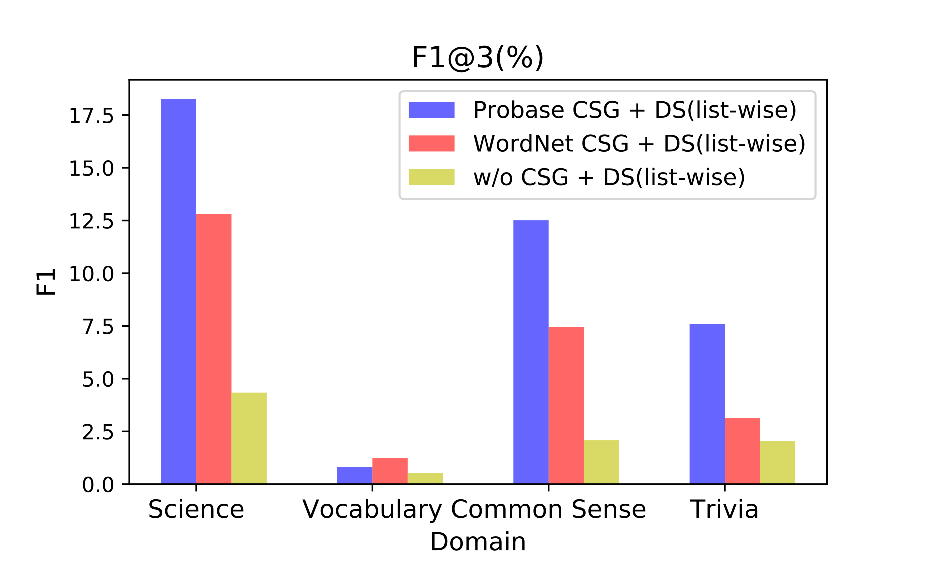
\epsfig{file=figure/f1.eps, width=0.45\columnwidth}
%}
%\hfill
%\subfloat[After Preprocessing]{
%\label{fig:preprocess:2}
%\epsfig{file=figure/pref1.eps, width=0.45\columnwidth}
%}
%\caption{Results of Preprocessing}
%\label{fig:preprocess}
%\end{figure*}
%% \KZ{There seems to be some repetition from the eval section.} 
%

In our system, two parameters are important for the 
performance. 
One is the parameter $k$ in the {\em Constraint} function 
\equref{equ:constraint}, which affects the weight of 
the spatial constraints.
Another is the threshold $t$ in the same function, which 
determines whether the input data satisfy the 
type and spatial constraints based on our scoring policies 
and how many candidates will be generated.  

%\JL{In our system, two parameters which should be defined by ourselves are very important.One is the parameter $k$ in the {\em Constraint} function 
%	\equref{equ:constraint}, 
%	which affects the weight of 
%	the spatial constraints in the whole set of constraints. Another is the threshold we set since an appropriate threshold could give us appropriate numbers of candidates after the selection by filtering some bad results.}
% \KZ{Which param in constraint. The constraint function needs to be
% defined carefully.}
In the implementation process, 
we hold out 20 images separately to train these two parameters 
and choose the ones that have the best performance. 
% some more results

Although our system achieves good results based on our 
experiments, there are some limitations that call for future 
work. First, in order to fuzzy match the information onto the images, 
we need to provide enough constraints in the description, 
such as the type of the 
data or the range of the data. If the constraints are not 
sufficiently specified, it is hard for our system to evaluate what 
data among the OCR outputs are more suitable for the description. 
For example, if we constrain the data to be an integer in the 
description, then any integers that appear in the OCR output can be 
candidates if they satisfy the spatial constraints. 
In many cases, insufficiency in the constraints can be 
made up by the constraints indicated from the neighboring descriptions. 
But sometimes, simple descriptions will lead to sub-standard results. 
Second, the correction model 
we generated is a probabilistic model based on the statistics. 
This correction model can make mistakes, 
e.g., correcting the right answer into the wrong one. More data 
from manual correction will help to reduce this possibility. 

% \KZ{Perhaps there's more issues you can discuss, now that u have
% changed the def of the correction model...}


\section{Related Work}
This section surveys previous works on question generation and tree encoding
respectively.

Text question generation has attracted the attention 
after the work of ~\citeauthor{du2017learning}~\shortcite{du2017learning}, who uses deep seq2seq model 
to generate questions from a raw text paragraph. 
Before that, text question generation relied heavily on hand-craft 
question patterns~\cite{HeilmanS10,LabutovBV15,MostowC09} which is time and 
labor consuming. 

However, this pure seq2seq model is not focused and 
has no control over part in the paragraph to generate question. 
~\citeauthor{zhou2017neural}~\shortcite{zhou2017neural} proposed to encode 
key phrase information using binary indicators to generate 
key-aware questions and they assumes the answer to be key phrase. 
Considering key phrase (answer) is unavailable in reality, 
~\citeauthor{SubramanianWYT17}~\shortcite{SubramanianWYT17} applied 
a two-stage approach. First, key phrases are extracted by 
pointer network~\cite{ptrnet}. Second, 
key phrases are encoded in the same way as 
Zhou et al. With the intuition that questions could be asked in many ways, 
~\citeauthor{Yao2018vae}~\shortcite{Yao2018vae} used conditional-VAE to 
increase the diversity of questions. More recently, models with 
auxiliary feature information~\cite{HarrisonW18} helped improve 
the question quality. Structure question generation aims at 
converting structured data such as triples in knowledge graph to questions. 
~\citeauthor{SerbanGGACCB16}~\shortcite{SerbanGGACCB16} proposed a model to generate factoid questions from knowledge base triples.  None of the above work
considered using parse tree structures to aid question generation process,
which is the focus of this paper.

Sequential RNN model takes sentence as a sequence of words, 
ignoring the syntactic information. In order to utilize
such syntactic information with sequential information, 
~\citeauthor{tai2015improved}~\shortcite{tai2015improved} proposed Tree-LSTM to 
encode the binary parse tree recursively in a bottom-up fashion to 
classify sentiment. In text generation task, 
\citeauthor{eriguchi2016tree}~\shortcite{eriguchi2016tree} 
proposed a tree-to-sequence model with attention mechanism to do 
machine translation and 
~\citeauthor{liang2018automatic}~\shortcite{liang2018automatic} proposed a 
tree-to-sequence model which could handle arbitrary trees, 
to do code comment generation. Our work is inspired by these previous
attempts and we are first to adapt structure encoded neural models to
textual question generations.
\section{Conclusion}
We implement a novel sequence-based dependency parsing
framework which takes advantage of high order features 
in parsing history. 
%We can also adapt beam search to this framework so as to
%relax the strictly greedy nature. Vine pruning\cite{rush2012vine} could
%be incorporated to speed up the parsing.
More importantly, we discovered that the parsing accuracy is very sensitive to
the quality of parsing sequence. Future work can be focused on
developing better sequence predictors that outperform Malt action classifier.
Furthermore, we use two sets of features for sequence predictor and
head mapper right now. A unified set of features between these two components
are worth exploring.
%Besides, better sequence predicting method and unified feature
%representation of two components are worth exploring.
%
%Though we currently get a not bad result,
%the sequence predictor still needs more exploration.
%According to our experiment, slightly changes
%on the sequence can lead to a fatal decline on accuracy. Ensuring the match degree of training sequence and testing
%sequence demands a high quality of sequence predictor.
%
%Further, the features in our current implementation are not expanded and well tuned yet  and we are free to define high order features to make use of parsing history. Our framework is flexible to merge other technics to enhance the performance. Introducing beam could make up for our greedy decoder and improve our accuracy. Vine pruning\cite{rush2012vine} could speed up parsing process. Besides, better sequence predicting method and unified feature representation of two components are worth exploring.


\section*{Acknowledgments}
Kenny Q. Zhu and Jia Wei are the corresponding authors. This work
was partially supported by the AstraZeneca-SJTU collaborative
research grant.

%% main text
% \section{}
% \label{}

%% The Appendices part is started with the command \appendix;
%% appendix sections are then done as normal sections
%% \appendix

%% \section{}
%% \label{}

%% If you have bibdatabase file and want bibtex to generate the
%% bibitems, please use
%%
\bibliographystyle{elsarticle-num-names}
\bibliography{ocr}

%% else use the following coding to input the bibitems directly in the
%% TeX file.

% \begin{thebibliography}{00}
%
% %% \bibitem{label}
% %% Text of bibliographic item
%
% \bibitem{}
%
% \end{thebibliography}
\end{document}
\endinput
%%
%% End of file `elsarticle-template-num.tex'.
